%NOTE: 
% [P#] = participant ID, 
% below [P#] like f2, e10 are the reference to the quote in the Google sheet 
%Quotes, Codes, themes :https://docs.google.com/spreadsheets/d/1Ot8ZtLUwnGUQWf-VQGgj-1pVSrVmZQ46KfvHWE6VxiE/edit#gid=0
    
    

\section{Results}
    We present our findings from a 4-weeks `in-the-wild' study regarding self-reports mental health and wellbeing via \ac{CA} involving $20$ participants with \ac{AD}.
    % 
    First, we report on the quantitative findings including  participant's personality types, their response to the \ac{UEQ} questionnaire, and adherence to the study protocol.
    % 
    We then present the our findings from the thematic analysis of the interviews including transcribed quotes representing the themes and sub-themes they discuss. The analysis of the interview data revealed six major themes on how the participants perceived self-reporting of mental health and wellbeing through speech-enabled \ac{CA}: 
        (i) Factors influencing conversational self-reports
        (ii) Perceived therapeutic effects of conversational self-reports 
        (iii) Influence of \ac{CA} limitations in conversational self-reports 
        (iv) Privacy perceptions and the concerns with conversational self-reports
        (v) Participant's social circle's opinion on conversational self-reports
    % 
    Lastly, we summarize the characteristics of a \ac{CA} that users envision to self-report their mental health and wellbeing.


    \subsection{Quantitative findings}

    
    \subsubsection{Personality traits} 
        
    \begin{figure}
        \centering
        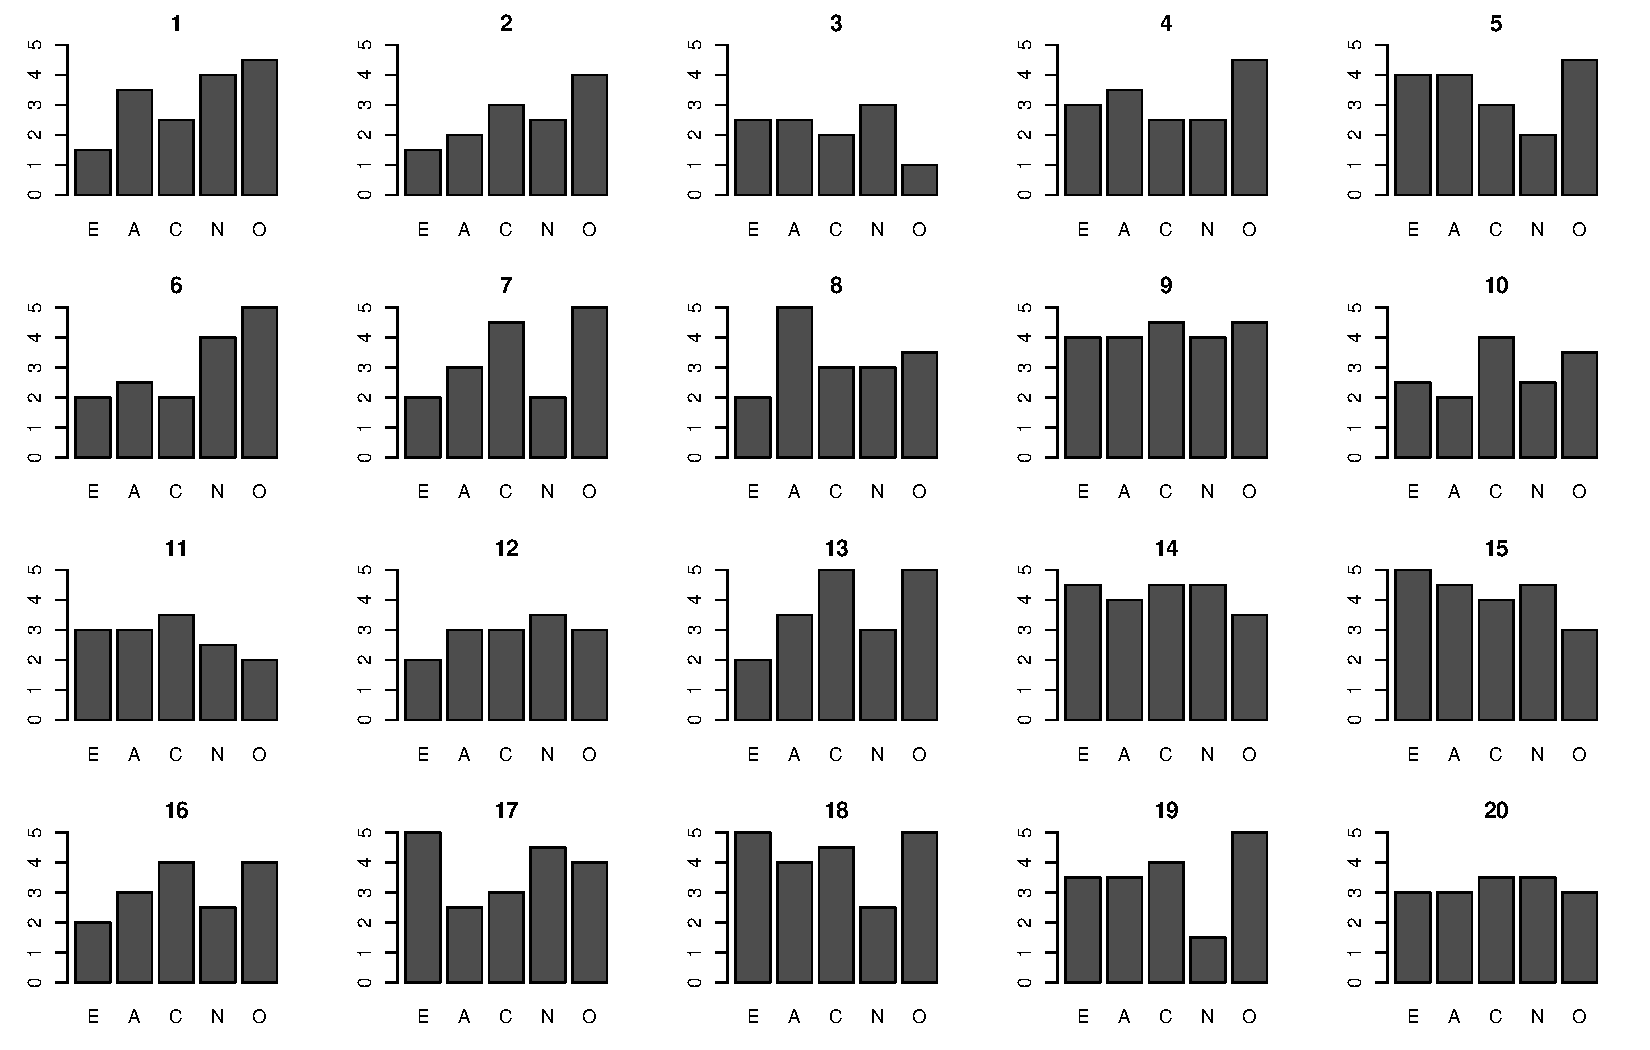
\includegraphics[clip, trim=0cm 0cm 0.25cm 0cm, width=\textwidth]{figures/personality.pdf}
        \caption{Personality traits of each participant based on \ac{BFI-10} questionnaire. X-asis represents each of the 5 personality traits where E = Extraversion, A = Agreeableness, C = Conscientiousness, N = Neuroticism, O = Openness to experience. Y-axis represents the participant's self-reported score on each trait.}
        \label{fig:personality}
    \end{figure}
     
    The overall personality traits of the participants in the study reflected as 
        extraversion    ($ M = 3.00, SD = 1.20 $),  
        agreeableness   ($ M = 3.30, SD = 0.80 $),    
        conscientiousness   ($ M = 3.50, SD = 0.89 $),    
        neuroticism ($ M = 3.10, SD = 0.91 $), 
        openness.to.experience  ($ M = 3.88, SD = 1.09 $).
    % 
    Figure \ref{fig:personality} illustrates each of the participant's personality traits based on based on \ac{BFI-10} questionnaire.


    \subsubsection{\acl{UEQ}}    
    \begin{figure}
        \centering
        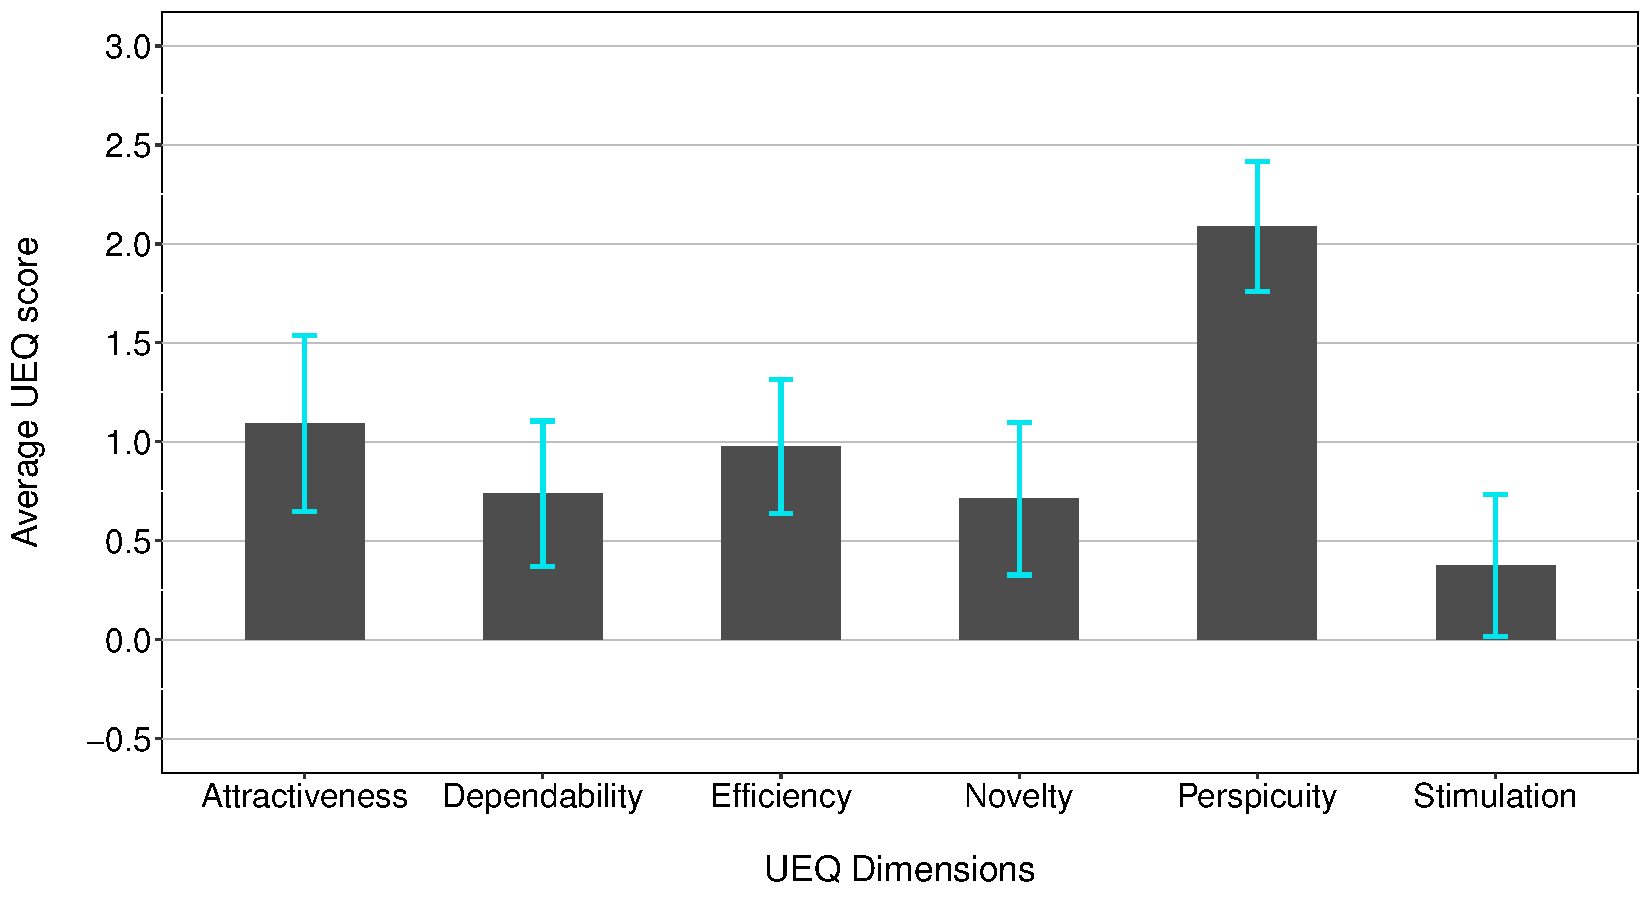
\includegraphics[clip, trim=0cm 0cm 0.5cm 0.5cm, width=0.8\textwidth]{figures/ueq.pdf}
        \caption{Participant's mean \ac{UEQ} score in each dimension with error bars reflecting margin of error.
        Values between $-0.8$ and $0.8$ represent a more or less neutral evaluation of the corresponding scale,  values $> 0.8$ represent a positive evaluation and values $< -0.8$ represent a negative evaluation.}
        \label{fig:ueq}
    \end{figure}
    % \begin{figure}
    %     \centering
    %     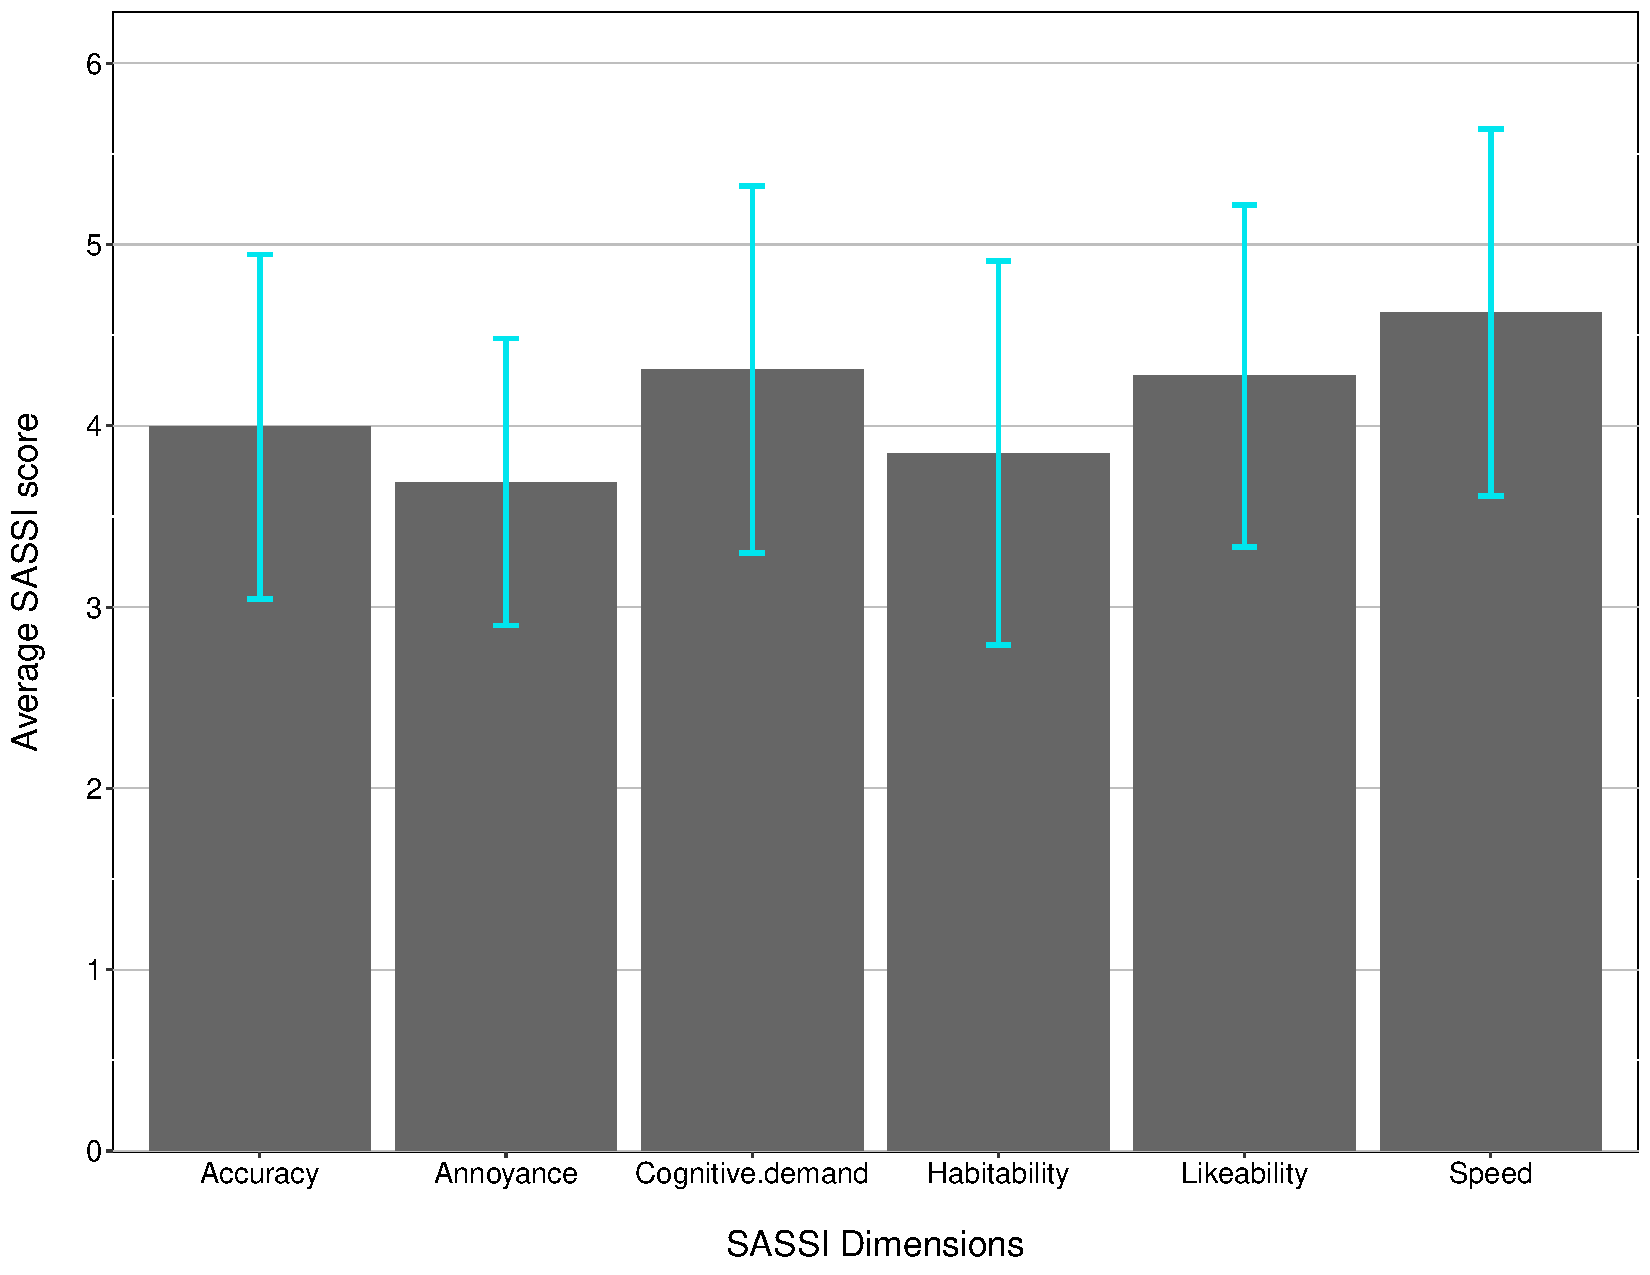
\includegraphics[clip, trim=0cm 0cm 0.5cm 0.5cm, width=0.45\textwidth]{figures/sassi.pdf}
    %     \caption{Participant's mean \ac{UEQ} score in each dimension with error bars reflecting standard deviation.
    %     Values between $-0.8$ and $0.8$ represent a more or less neutral evaluation of the corresponding scale,  values $> 0.8$ represent a positive evaluation and values $< -0.8$ represent a negative evaluation.}
    %     \label{fig:ueq}
    % \end{figure}

    In general, participants expressed positive experience self-reporting their mental health and wellbeing despite technical limitations. 
    % 
    Figure \ref{fig:ueq} shows participant's impression of their self-reporting experience via \acl{app} in terms of
        Attractiveness ($U = 1.09, SE = 0.44 $),
        Perspicuity ($U = 2.09, SE = 0.33 $),
        Efficiency ($U = 0.98, SE = 0.34 $),
        Dependability ($U = 0.74, SE = 0.37 $),
        Simulation ($U = 0.38, SE = 0.36 $),
        Novelty ($U = 0.71, SE = 0.38 $).
    % 
    The figure shows participants' positive perceptions of perspicuity and attractiveness, indicating \ac{CA}'s strong potential in supporting engaging self-reports of mental health and wellbeing. Their neutral view on dependability, efficiency, novelty and simulation of self-reports via \ac{CA} suggests the need for design and technical improvements.


    \subsubsection{Adherence}  
    \begin{figure}
        \centering
        \includegraphics[clip, trim=0cm 0cm 0.15cm 0cm, width=\textwidth]{figures/adherence.pdf}
        \caption{Participants' adherence to daily self-reports of mental health and wellbeing via \acl{app}.Each dot represents an entry for the day. Annotations reflect each participant's adherence rate during the study duration. The red bar indicates Dialogflow's service outage on August 20, 2020. Participants were not able to use \acl{app} on that day.}
        \label{fig:adherence}
    \end{figure}
    
    Analysis of the timestamps collected through \acl{app} shows that the average participants' adherence rate to self-report was $74.64\%$ which is comparable to prior studies implementing \ac{EMA} in mobile devices~\cite{wen2017compliance}. Figure \ref{fig:adherence} illustrates the summary of the participant's adherence to daily self-reports during the study period. 
    

    
    % in relation to the
    % perceptions of people with \acp{AD} on self-reporting of mental health and wellbeing via speech-based \acp{CA} and the \ac{CA} design characteristics they see as important to support long term conversational self-reports.



    %NOTE: 
    % [P#] = participant ID, 
    % below [P#] like f2, e10 are the reference to the quote in the Google Sheet:https://docs.google.com/spreadsheets/d/1Ot8ZtLUwnGUQWf-VQGgj-1pVSrVmZQ46KfvHWE6VxiE/edit#gid=0



\subsection{Factors influencing adherence to self-reports via \ac{CA} }
        
    Participants' narratives indicate that smart speakers' mobility and users' mental, physical, and cognitive issues are the primary reasons for non-adherence. Additional factors contribute to the non-adherence for some.
    % 
    Participants compared other forms of self-reports and suggested that convenience and speech-based interaction are the main factors to facilitate conversational self-reports.

    
    \subsubsection{Barriers to adherence}
        While our results indicate participants' strong adherence to daily self-reports, participants reported mobility of the smart speaker and their own mental and cognitive issues as the primary barriers to self-reports via \ac{CA}.
        
        
        \textbf{Smart speaker's mobility. }
        Unlike smartphones, smart speakers are designed for home use and require continuous power supply and Wi-Fi connection.
        Most participants in the study used the system at their home and reported that they mostly talked to \acl{app} in the evening. 
        While most participants expressed that talking to \acl{app} about their mental state at home made them feel safe and comfortable, 
        % \begin{quote}
        %     \textit{
        %     So I definitely like the fact that I,  really like the fact that I wasn't really confronted with these questions, when I was, anywhere else but home.
        %     % It was sometimes it would be really, when I had the app like it would it would like notify me three times a day and sometimes I would be in a place where I'm actually, I feel quite good and then it was like telling me to do these things and like, And 
        %     I also feel like it's really nice to like be in a nice environment where you feel safe when you have to share these thoughts and so on.
        %     }
        %     [P12]
        %     % p23        
        % \end{quote}
        % 
        many participants stated that due to the smart speaker's static nature, they were not able to use it when they were away from home.
        % \begin{quote}
            \textit{``I think it happened twice and was the days where I wasn’t so much home.''}
            [P17]
            % u23
        % \end{quote}
        
        % 
        % \begin{quote}
        %     \textit{
        % Some days just because I didn't want to, just want to go to sleep, no energy to talk. Somebody just because I wasn't just not at home, like, there was a weekend, traveling etc. Some days I was at my boyfriend's place.
        % }
        %     [P8]
        %     % l23
        % \end{quote}
        
        % \begin{quote}
        %     \textit{
                % So I would speak every day, but maybe some days I would forget, like two days. Okay. Or I wasn't home for two days. No. And then or maybe, yeah. And then. And then maybe one day I would forget during the week, and then I would try to do it every day. But maybe two days I forget and then or not forget, I wouldn't be home. And then, like one day, I wouldn't just do it. Yeah, it's just like, yeah, those were the reasons like I wasn't home or I forgot.
                % }
        %     [P11]
        %     % o23    
        % \end{quote}

        Despite the static nature of the smart speaker, P14 and P6 however, took the smart speaker with them when they were away from their home and described that it was not much of a hassle to set up the system in a new place as long as they had access to the electric outlet and Wi-fi.
        % Participants P14 and P6 on the other hand, took the smart speaker with them when they were away from their home and mentioned that 
        % \begin{quote}
            \textit{``So for three weeks I was in the sort of caravan that close to the factory that I was doing samples. And, yeah, actually it worked fine. I just had to reset it to my, to the Wi-Fi, and that was not a problem.''}
            % [P14]
            % r27
        % \end{quote}
        
        % \begin{quote}
        %     \textit{
        %     % I would like to say also really really like how I can pick up the Google Home and just bring it everywhere. I didn't really think of this but like 
        %     I had to go to my in laws for a couple of days... 
        %     % And at first I was thinking oh no I am participating in this project 
        %     and it's like, oh wait it's not hard I just pick it up and I plug it in, in a new place.
        %     % and then I just continue where I left off. 
        %     And it was really nice. It wasn't any hassle. It wasn't a lot of effort you had to put into it you just plug it in anywhere you go. And I've been thinking a lot about this past week how, if I had to continue with something like \acl{app} I would probably bring her (smart speaker) everywhere. 
        %     }
        %     [P6]
        %     % j27
        % \end{quote}
        % 
        \textbf{Users' mental state. }
        % ----mental and physical state----
        % Participants described that their mental state also affected their adherence to self-reports. 
        Participants described that their mental state of mind affected their social interaction, which included talking to \acl{app}.
        %   
        P16, who suffers from bipolar disorder, for example, mentioned that they felt comfortable talking to \acl{app} when their mood is elevated but refrained from talking to \acl{app} reflecting their loss of interest--a symptom of a depressive episode--when they were depressed quoting,
            % \begin{quote}
                \textit{``When I'm up, because I have bipolarity. Sometimes I'm up and sometimes I'm down. When I'm up. It's okay. I'm completely comfortable with \acl{app}. It is nice, but when I'm down, I've been down. I don't want to talk to her at all.''}
                % [P16]
                % t23
            % \end{quote}  
        % 
        Likewise, P1 stated that when they are depressed they tend to cease social activities like talking to people, including talking to \acl{app}, noting:
            % \begin{quote}
                \textit{``When I am quite down, I close down. I don’t talk to anyone. It’s not just \acl{app} I mean.'' 
                % From time to time, I was either down and I didnt want to use \acl{app}. Or during the time I was living with my boyfriend and it was difficult for me to ask him to leave the room as I want to use \acl{app} when I have time and privacy. At one time, I wasn’t in town. Also may be because I didn’ t use the alarm clock to remind me. 
                }
                [P1]
                % e23
            % \end{quote}
        % 
        Participants also mentioned  that sometimes they just did not feel like talking to \acl{app} due to their emotional state at the end of the day. P4 said,
            % \begin{quote}
                \textit{
            %     I think I did. Okay. I had to. At the time when I was in Germany, and then I had a weekend where I was at the [social event]. And      then I didn't talk, 
                ``I think I had some evenings, I think it was like I had like really rough day, I just forgot because I was so tired.''
                }
                % [P4]
                % h23
            % \end{quote}    
        
         
        \textbf{Cognitive issues. }
        % ----Forgetfulness----
        Forgetfulness surfaced as another reason for non-adherence to daily self-reports. Prior studies have demonstrated that notifications or reminders are an effective method of increasing user adherence to self-reports.~\cite{moller2013investigating, hofmann2015surveysignal}. While \acl{app} did not automatically send notifications to self-report about their mental health and wellbeing every day, participants were informed on setting up a reminder in Google Nest and encouraged to use this feature to remind themselves to talk to \acl{app}. More than half of the participants ($n=12$) used this feature and asked Google Assistant to remind them to speak to \acl{app}.
        % 
        Participants were also introduced to the `routine' feature in the Google Assistant which triggers multiple actions with a single phrase\footnote{\url{https://support.google.com/googlenest/answer/7029585?co=GENIE.Platform\%3DAndroid&hl=en}}. 
        % Only one participant used this feature.
        
        Participants found it very simple to set up the reminder. However, many participants canceled the reminders later in the study as they found them intrusive and irrelevant in some cases.
        % 
        P4 for example, shared an uncomfortable incident when the reminder went off when they had a friend over with whom they might have not shared about the study otherwise.
            % \begin{quote}
                \textit{``I set it like once or twice, where it went off, when I was like, I think I had a friend over or something... like, `Hey, see this' and I did actually talk to her, but it was like, like `I'm doing this study' and people were like `what?', `you're supposed to do what?', `you're supposed to tell him about the day?' 
                % But it's like also so quick so it's just like poof, and then you're done, like. 
                That was weird. And I told him that I am in a study on testing technology.''}
                % [P4]
                % h24
            % \end{quote}   
        % 
        For P3 and P12, the reminder they set up at the beginning of the study quickly became obsolete as they were mostly not at home at the time they had set up the reminder.
            % \begin{quote}
            %     \textit{In the beginning I did set up notification but then I found that I wasn’t home all the time. }
            %     [P3]
            %     % g23
            % \end{quote}
            % \begin{quote}
                \textit{``Most of the days I wasn't really in my dorm room when I got the notification.''}
                % [P12]
                % p24
            % \end{quote}
        
         
        Participants who did not set up the reminders described that the notification was not necessary for them as they were able to remember to talk to \acl{app} on their own. 
        % 
        % ----physicality----
        % 
        P5 and P8 mentioned that the physical presence of the smart speaker reminded them of the self-reporting task. P5 noted: 
            % \begin{quote}
                \textit{``Sometimes I look at it and I am reminded.''}
                % [P5]
                % i24
            % \end{quote}
            % 
            % \begin{quote}
            %     \textit{I started to use the Google Assistant for different things, alarm in the morning, setting an alarm for cooking pasta, this kind of things. So I knew, it was there, I knew, I at some point I had to talk. 
            %     % I mean it's so, it's not, it's accessible, it's nice, it's accessible, that I think about it and then I can just say, 
            %     So I didn't have to put any notification.}
            %     [P8]
            %     % l24
            % \end{quote}
        % 
        % ----Intrusive----
        P11,  who did not set up a reminder to talk to \acl{app}, perceived \ac{CA} notifications intrusive. They explained that they did not set up the reminder to talk to \acl{app} as wanted to self-report their feelings when they are ready without feeling forced to do so.
            % \begin{quote}
                \textit{``The thing is, I, I think one of the reasons is because, like, I don't know, that would feel like I am being forced to express my feelings, as opposed to expressing my feelings whenever I wanted you know, like, you should talk to \acl{app}. And you do it when you're you feel ready, you know?''}
                % [P11]
                % o24
            % \end{quote}    

         
        \textbf{Additional factors for barriers to adherence. } 
        In addition to the smart speaker's mobility, users' mental state and cognitive issues, (i) need to remember the invocation phrase ($n=2$), and (ii) privacy ($n=1$) also emerged as factors for non-adherence to conversational self-reports. 
        % 
        Two Participants, P2 and P7 reported that at times they had problem remembering the invocation phrase to use \acl{app}. However, they were able to remind themselves by looking up to the documentation provided. P7 said,
        % \begin{quote}
            \textit{``I think there was one time that I forgot the command, so I had to look up.
            % 
            But I was really, really, really tired when I came back for work and my brain was totally toast. But that's the only that's the only problem and that she was, she was really too She was really effortless to work with.''}
            % [P7]
            % k52
        % \end{quote}
        % 
        P1 was accompanied by their partner many days during the study period. During the period of their partner's presence, they did not feel comfortable talking to \acl{app}. As a result, they were able to self-report for only $32\%$ of the days.
        

        
        
    \subsubsection{Facilitators to conversational self-reports}
        %
        Most ($n=15$) participants in the study had self-reporting experience through other media such as mobile and web apps and paper journals.
        Participants often compared their self-reporting experience via \acl{app} with their prior experiences.  
        They described that self-reporting via \acl{app} was more convenient, cognitively less burdensome, and perceived that the conversational form of interaction with \ac{CA} was more natural than other forms of self-reports. 
        These characteristics of \ac{CA} could have facilitated self-reporting via \acl{app}.

        \textbf{Convenience. }
        In line with the prior findings on the general population's adoption of smart speakers~\cite{lau2018alexa}, participants in this study indicated that one of the primary factors for users to self-report via \acl{app} was the convenience offered by \ac{CA}.
        % 
        Unlike other forms of self-reports (e.g., on pen and paper, and through web or mobile apps), participants do not have to prepare any tools to self-report via \ac{CA}. Participants found this hands free interaction to self-report their emotions via \ac{CA} convenient. P1 noted:
        % 
        % ----don't have to log in open laptop/notebook----
        % 
        % \begin{quote}
            \textit{
            ``I think I love it because it’s like an interface you talk directly to. You can just talk to it. It’s super easy to use. You don’t have to open your laptop and go to a specific page. I can just go home, open the door and talk to \acl{app}, super easy.'' 
            }
            % [P1]
            % e25
        % \end{quote}
        
        % \begin{quote}
        %     \textit{
        %     It encourages people, 
        %     % so make it as easy as possible, 
        %     because sometimes using apps you have to open your phone, you’ve to think about it. With this one, you can just walk into your room and say `Hello \acl{app}' and talk to it. 
        %     }
        %     [P20]
        %     % x25
        % \end{quote}

        % \begin{quote}
        %     \textit{
        %     Somehow you know its not same like with a person, but you get used to talking to it because you do it daily right so it gives me certainty after having dinner I, its sort of like a habit now which was quite impressive because the other one when I had to write it down, 
        %     % it did not work very well because I did not get reminder and 
        %     it was much more difficult. \acl{app} was there already. I didn’t have to log in. It was easy. 
        %     }
        %     [P14]    
        %     % r25
        % \end{quote}
        
        % \begin{quote}
        %     \textit{
        %     I thought I thought it was actually it was very easy. You know, it was like, it was very clear from the start, like what \acl{app} was about. And it was simply just starting \acl{app} up and just talking. And that was super easy.
        %     }
        %     [P11]
        %     % o26
        % \end{quote}
        % 
        P2 and P3 found talking to \acl{app} from the comfort of their bed relaxing. P3 noted: 
        % \begin{quote}
            \textit{
            ``Talking to \acl{app} is more simple as well. If you lay in your bed and you're like, Oh, I haven't to talked to \acl{app} today, you don't have to then open your computer again and start writing until late. You can just lay in your bed with closed eyes and finish off talking to her.''
            % Also, as I said, it's, it's limiting and thereby less time consuming, as well, that sense. Also because there is that response, instead of you pouring your heart out into this long block of text, you at least get some sort of response.
            }
            % [P2]
            % f25
        % \end{quote}
        
        % \begin{quote}
        %     \textit{
        %     I like talking rather than writing. 
        %     % So that was great. 
        %     You can just lie down on your bed and start talking to \acl{app} so that was relaxing.
        %     }
        %     [P3]
        %     % g25
        % \end{quote}


         
        \textbf{Reduced cognitive burden. }
        Participants perceived self-reporting via \ac{CA} less burdensome than writing. 
        They explained that speech-based self-reporting is often spontaneous which requires them to think less about the semantics.
        % 
        % spontaneous
        P7, who identified themself as an introvert and found writing much easier than speaking, 
        perceived self-reporting via \acl{CA} spontaneous, cognitively less demanding and provided them immediate emotional relief than when they wrote, quoting,
            % \begin{quote}
                \textit{
                % Like I said, in the beginning, it was really hard to realize you know that you have to speak here at now. 
                ``I'm an introvert. For me, writing is a lot easier than speaking. 
                % So it was actually really nice and interesting to get myself challenged to speak to her on a daily basis. 
                % But yet the whole breaks thing was really a hindrance the the first couple days, I think, but after that, it was it was cool.
                Remembering from when I when I journaled back in the days, talking to \acl{app} provided a more immediate emotional relief compared to writing. 
                Because, you know, writing is a lot slower than speaking, especially by hand, and you know, and the entire time that you're writing, you're actually mulling those feelings over. You are looking for the right expression, you know, concentrating on the handwriting and stuff. 
                With with \acl{app}, you know, you just get it out of the system. Like, like, here, it's out. 
                % It's so good now, and it doesn't bother me as much anymore. 
                Plus, it's a lot more spontaneous. 
                % I think I tried to keep myself very civilized, even though I really wanted to cuss many days. But \acl{app} is not ready for that yet.
                % 
                I think \acl{app} is great for capturing and the immediate responses of the emotion because you don't have to have to think about it. 
                You don't have time to formulate it, use it, just get it out there. Meanwhile, in writing, you know, like, like, we just said, you know, you might look, you might write something and feel that was just, like, too intense. 
                It's like, Oh, this is like, such a bad thing to say, Does this make me a bad person to use? Like, scratch it? to start over?''
                % 
                }
                % [P7]
                % k26
            % \end{quote}
        % freedom of expression
        P14 shared similar views on talking to \ac{app} about their feelings and perceived speaking as a more free form of expression than writing. They mentioned that while \ac{CA} allowed them to talk freely about their feelings, writing about feelings often got lengthier, which demotivated them to continue self-reporting.
        % 
            % \begin{quote}
                \textit{
                % it's what's actually much better than writing it down because then I just felt, I can just freely talk and I don't really need to think about what I write down. And I can just say what comes to mind and sometimes you have when you have to write it down you really have to think properly about what you write down and sometimes it cannot be as spontaneous as I would say.
                % 
                ``Speaking is much easier because you can just let the words flow and you don't have to think about it and when you're writing it sometimes if something takes really long to write down You think I'll just leave it and not write it down. So in that way, speaking is better for sharing my thoughts I think.''
                }
                % [P14]
                % r27
            % \end{quote}
        % obligatory/stressful
        They further added that writing about their feelings felt obligatory and stressful, therefore preferred talking to \acl{app} as it took less time for them to express their thoughts.
        % 
            % \begin{quote}
                \textit{
                ``Whenever I wrote stuff down, it felt more like, I don't know, it felt more like an obligatory thing. And now it was more nice with \acl{app} because it's only a couple of minutes, and then if I had to write stuff down I had to sit for it and then I felt like more of a pressure on what I have to write.''
                }
                [P14] 
                % r26
            % \end{quote}
            % 
        % Likewise, P16 and P19 shared their experiences writing a diary describing their lack of control over their self-reports resulting in an excessively long log of daily activities. In contrast, they found talking to \acl{app} spontaneous and perceived more control over their self-reports.
        % P16 said,
        %     % \begin{quote}
        %         \textit{
        %         ``I tried to have diaries and I was I don't know 15/16 years old at that time but then when I started to write my diaries, then I realized I have written more than five pages. But diary is not your full story diary is something, like an abstract of your day. And then, after, after I don't know two or three days, then I decided to stop doing that.
        %         ...
        %         If I have to compare \acl{app} with writing down the diary, \acl{app} is better, because when you want to write down something you need to be comfortable you need some paper you need a pencil to write, then you need to think, then you need to write. And when you write, sometimes you cannot stop. Sometimes you say okay I'm tired of that. But when you have some voice interaction, then you don't need to think more and you don't need to have any setup, you just start talking. And you can stop whenever you want.'' 
        %         % 
        %         }
        %         % [P16]
        %         % t25
        %     % \end{quote}
        % 
        % Writing is too formal
        P20 perceived writing about their feeling as a formal process during which they often contemplated what they should write and ultimately did not write anything. They found self-reporting via \acl{app} informal, which made it more like talking to a person.
            % \begin{quote}
                \textit{``Personally, when I’m talking, I’m a lot less filtered. While writing down, it feels more formal - it’s a lot concrete, I press myself to think and I end up not writing my thoughts thinking that it’s not good to think that. When you’re talking, it's a lot more personable, maybe something you say to someone you know.''}
                [P20]
                % x26
            % \end{quote}
            
            
        % Finally, P19 described that although they suspected that talking to \ac{CA} would not be different than writing a diary, they stated that they felt more fluent and found \ac{CA} more accessible way of self-reporting.
        % \begin{quote}
        %     \textit{
        %     In the beginning and they felt that it was just gonna end up being a diary, like just another diary, which with the written one, it was pretty much just a diary, which isn't a bad thing. I liked writing my diary back when I did that myself. The spoken one, the, the Google Home one. It felt it felt more fluent in a way I don't know if you know what I mean with that. It felt more like I could just do it whenever I wanted to. So it's not something that I had to, for example, sit down and take a long time doing.
        %     }
        %     [P19]
        %     % w26
        % \end{quote}

        
        % \begin{quote}
        %     With the written one you got to go way more into detail. And you have to express, you got to think the entire day through in a way. Whereas, with the, the vocal one. You only kind of got to talk about the highlights, or, like, more expressing point. 
        %     But if I felt like I was missing something I would just have done another one in the same day, so it doesn't like if if you feel like you don't get to say enough then you could just do another one.
        %     [P19]
        % \end{quote}    
        
        
        
        
        \textbf{Natural form of interaction. }
        Participants stated that speech as a more natural form of interaction enabled them to express their emotions better, as they felt talking to \ac{CA} more like having a conversation with another person.
            % \begin{quote}
                \textit{
                ``It's feels more like a conversation with another thing, person. It felt more like a conversation than writing a diary because diaries, you're writing to yourself.''
                % , and even though I do write and draw a lot. I can still be a little impatient with myself in terms of how fast I'm writing. It's like you think much faster than you write of course, it's much better on a computer but the computer doesn't feel very human, to me, because it's like, you know. Oh, it's on a computer who doesn't too personal. So, I prefer writing it but then it's too slow so this is actually that was nice. If she. If there was like a program where she wrote all the things we were talking about into like this styrian form, then that would be pretty great, I think, because I like the fact that I could just talk in my normal rhythm and like fast and then I had the recollection recorded.
                }
                % [P18]
                % v26
            % \end{quote} 
        % 
        People with \ac{AD} are often asked to maintain a journal for clinical evaluation. Thus they view journaling as a clinical tool. 
        P10 perceived talking to \acl{app} less clinical than writing. They expressed that if they were in a depression, they would prefer talking to \ac{CA} because they find it easier and more personable than writing a journal.
        % 
            % \begin{quote}
                \textit{``I think it's easier, somehow, it's more natural and less, less clinical. It's more personable, in some way.
                It feels more personal with \acl{app}, in some way. It was easier. Definitely, like, I could see myself if I was deep into depression, then there was this would be a lot easier for me to to get around to doing than writing something down.''}
                % [P10]
                % p26
            % \end{quote}    
        % 
        Furthermore, P11 mentioned that as speaking is an easier method of communicating one's feelings, it might be a good starting point for people who do not communicate their feelings, quoting,
            % 
            % \begin{quote}
                \textit{
                ``I certainly think it's a much more natural way of expressing yourself as opposed to writing. 
                So in that sense it's easier to communicate your feelings, which might be a good thing for people that don't have experience communicating their feelings.
                % and maybe starting to write is not the best way, but instead to speak, because it's just quite easy and quick.''
                % But maybe after realizing the impacts of speaking, and how good it feels to release. Yeah. Or, like, likes, yeah essentially how how it makes you feel good by speaking your feelings. 
                % Maybe they might move to writing as well. Yeah.
                }
                % [P11]
                % o26
            % \end{quote}
            
        

\subsection{Perception on conversational self-reports}
% \acl{CA} for Emotion Regulation
    
    Participants described several therapeutic attributes that they valued in self-reporting their mental health and wellbeing via \ac{CA}. 
    % 
    They perceived \acp{CA} as an effective means of emotion regulation. 
    % 
    In particular, participants liked the fact that they could vent their emotions aloud to the \ac{CA} without any judgments and repercussions.
    % 
    Participants also stated that they found \ac{CA} more approachable than humans to express their feelings and found talking aloud with \ac{CA} therapeutic.
    % 
    Most of the participants personified \ac{CA} in different ways and shared its potential as a companion and digital therapist.
    % 
    Further, participants reported that talking to \ac{CA} facilitated self-reflection.
    
    % due to its inherent characteristics that 
    
    % Both the therapeutic effects and the users perception on the role it could play in providing emotional support and counseling. 
    
    \subsubsection{Conversational self-report as emotional venting}\label{sec:emotional_venting}
    Emotional venting is considered an effective way of finding relief by releasing strong or repressed emotions~\cite{bennett1991irrationality, tonnaer2020explosive, leslie2008boxing}. 
    Participants characterized self-reporting their emotions via \ac{CA} as a way of emotional venting. 
    % 
    They described \acl{app} as a good listener and that it allowed them to express their emotions without any judgment and repercussions.
    % 
    They stated that they simply felt relieved when they expressed their feelings aloud.
    


        % Participants perceived \ac{CA} an effective means of emotional venting. 
        % WHY CAs ARE EFFECTIVE TOOL FOR EMOTIONAL VENTING? 

        \textbf{`Sometimes all you need is someone who listens'. }
        Participants mentioned that it is often challenging for them to communicate their feelings to others, including their loved ones in the family or health professionals. When they express their feelings, listeners are often too keen to understand the situation and their problems in an attempt to solve their problems, which is not what the participants expect.
        
        % ---- No judgment ---- 
            P4 For example, compared their experience sharing their feelings with humans and talking to \acl{app}. They expressed that they liked the fact that they were not judged, quoting,
            % \begin{quote}
                \textit{``I think, you cannot compare it to this conversation with someone, of course, which is more comfortable I would say. But in some way, it's really nice because you don't get advice like from people, because I know that's especially if I share that I'm quite stressed, then people say like, `Oh, then you have to, you know, go home a bit earlier' or 'You can do this' and, and of course that's not really working for anxiety in like those kind of problems so it can be quite nice to just have no judgments or something like that which I really liked about it (\acl{app}).''}
                % [P14]
                % r4
            % \end{quote}
            
            % \begin{quote}
            %     \textit{    
            %     This is going to be a bit personal but the since this study that I have to go to the doctor and I have to get a. What's it called, they jam something up your butt to get some tissue from the inside of you. Okay. And it was a really unpleasant experience and it was like so much when I attend to the doctor, it wasn't pleasant but you don't feel like telling your friend oh I have a machine jammed up my butt so I can't sit down ... you don't really feel like telling your friends like that. But when I got home and it was like, I started to \acl{app} and she was like, how are doing, do you think extremely bad. Please tell me more. The doctor jammed something up my butt `aahahahhahah!!!' I think let's just the next sentence I said, because she doesn't care like you could tell her anything you can tell her about your sex life you could tell her how you feel, violent thoughts or anything it's not like she's going to tell you it's not like she's going to judge you or anything.
            %     }
            %     [P6]
            %     % j13
            % \end{quote}
            
        % ---- No unwanted solution ----
        Many participants shared that they often do not need a solution to their problems. Due to their mental conditions' chronic nature, they know how to cope with the situation or overcome their mental state. Therefore, they valued being heard than having their problems solved. They perceived \acl{app} as `someone' that made them feel heard -- a quality that is fundamental for sustainable long term \ac{CA}-user relationship.
        % 
            % \begin{quote}
                % \textit{``If \acl{app} can do, not to automate the life, to be someone to talk to. Yes, I can do that everyday. I can trust to talk to \acl{app} everyday. I don't know if you have ever seen the movie, `Her'~\cite{spike2014her}. Something like that. The `Her' thing is not to automate your life or to remind you anything. Google Assistant can do that. Someone to talk with, not to talk with to get your feedback, just to talk with to review your day and to see okay what you're actually doing.''}
                % [P16]
                % t5
            % \end{quote}
            % 
        P2 said, 
        % imagined themselves sharing their feelings with Google Assistant (considering it smarter than \ac{app}) 
            % \begin{quote}
                \textit{
                ``It sounds a bit stupid to say but I could say that I'm glad someone listens, except you know there isn't actually someone that listens. But it feels like it. Or at least I get to get some stuffs out. If you just need someone to vent out, you can, with \acl{app}''.}
                % [P2]
                % f2
            % \end{quote}
        % They also expressed that they would reject the response form an agent, noting:
            % \begin{quote}
                % \textit{
                % % ----
                % I think if I were to talk to Google Assistant about my feelings, then it would probably just search it up on the internet and say, why am I feeling sad, and then it's like `This web app says that', and you're like  `I don't care'. I didn't necessarily need an answer. I just needed to get it out. In that sense, \acl{app} is better that it doesn't actually give a proper response but it just listens. And sometimes all you need is someone who listens than have an answer.
                % }
                % [P2]
                % f2
            % \end{quote}
            
        Likewise, P6, who suffers from schizophrenia, expressed that they would appreciate a compassionate feedback rather than any help from people or through \ac{CA} when they have episodes like auditory hallucinations.
        They said,
            % \begin{quote}
                \textit{
                % I haven't talked about much about my schizophrenia, but 
                ``I suffer sometimes from auditory hallucinations where I like hear voices. And sometimes when I'm like in a room, working on projects. Sometimes I have to tell people like `I'm sorry. I'm distracted right now. I'm having a small episode. Please don't mind it'. And people really really want to help, and they want to understand. But it's just not what you need in that moment. You just need someone to say `Okay. That's okay. You feeling something and that's okay', `You're experiencing something and that's okay'. Because when you have a diagnosis like this, you also know that talking doesn't make it go away, but sometimes getting assurance `Okay, it's okay to feel, it's okay to experience what you experienced', that helps a lot. 
                And in that regard \acl{app} doesn't ask, she doesn't require you to explain anything. She just asks you how are you feeling. And if you want to tell them more you can tell them more and if you don't want to, you can just say I'm feeling sad, and that's it. In that aspect, she is a listener. Sometimes a listener is exactly what you need in a situation like that.''
                }
                % [P6]
            % \end{quote}
            
            % \begin{quote}
            %     \textit{
            %     As I mentioned, sometimes all you need is someone who listens and not actually answer. It's like that with people as well in general. Sometimes you just need to get to get everything out and not them to try to solve anything because there's not necessarily anything to solve, you just need someone to, to share your thoughts and feelings so that you are not alone. And In that sense, \acl{app} listens to that. And the `thanks for sharing'... it's the same reply that I mentioned earlier as well you don't necessarily see it as that. It's still. Someone who listened.
            %     }
            %     [P2]
            %     % f10
            % \end{quote}
            % 
        % "But for me, because I have this already for a very long time. It's just, it can be really demotivating if people just saying yeah you can just do this or you can just, you need to relax more or you need to do this and it's sometimes I feel like they don't really understand the problem because the problem is not that if I just don't do this anymore then it will go away. And, and it's just nice to be not able to get this feedback or something like that.
        % [P14]

        
        % \textbf{No repercussions:}
        Participants also expressed that not having to think about the repercussions of the listener's reaction, their interest in the subject matter, or their feedback provided a safe space for them to vent out their emotions. P14 said,
            % \begin{quote}
                \textit{
               ``It was very easy for me to talk to \acl{app} because it's like someone that doesn't, I mean, if you talk to a human, it can sometimes be that you can feel that they are not interested or may be you don't want to give them all your problems so to say, and with something like this [\acl{app}] it's quite easy because it's like a computer right so you don't have to think about someone else's feelings in this way...And for me, it's just nice to talk to someone that doesn't really bother about what I say.''
                } 
                % [P14]
            % \end{quote}
        % 
        P7 who suffers from \acl{PMDD} mentioned that sharing their emotions with others often often felt unwelcoming. 
        They described that talking to \acl{app} felt welcoming and caring, quoting,
            % \begin{quote}
                \textit{
                ``You know, my dysphoria (\acl{PMDD}) often makes it so that I think that I'm a bother to people, like `it's really annoying to listen to you bitch'. But since I knew \acl{app} doesn't mind, I felt it in some instances in a twisted way, I felt like she cared, like she was always there no matter how negative or positive I was feeling.''
                } 
                % [P7]
            % \end{quote}
        % 
        
        % ---- Trust ----
        % Participants mentioned that this judgment-free and repercussion-free self-reporting environment created a trust and encouraged them to open up.
        Due to the \ac{CA}'s affordance of this trustworthy conversation, participants found \ac{CA} more approachable than human counterparts. They perceived \ac{CA} as a harmless machine that cannot turn against them no matter what they shared with it. P7 said,
            % \begin{quote}
                \textit{
                ``I have massive trust issues. You know, it's probably about my upbringing. You know, I come from a family where I was not exactly allowed to be myself. I was not exactly listened to. So it's when you when you live in that condition for so many years, you kind of like grow up thinking that, you know, whoever you tell anything to they will use it against you. And so it's kind of like a self guarding mechanism. But you know, since I know that \acl{app} is a machine, she doesn't really think that much of herself and she's just there sitting on my table. That kind of makes it a little bit more approachable.''
                }
            %     [P7]
            % \end{quote}
            % 
            % \begin{quote}
            %     \textit{
            %     Because a lot of time, When you suffer from depression, it's also this thing where you can sit in a room full of people. And you can just say I feel sad. It's it's just creates this really strange atmosphere. And a lot of people know how to suffer from mental problems, and still it's really hard to just say oh I'm feeling sad right now I don't know why. It's just some feeling. But it's, it's not hard when you have something like \acl{app}, you could just go and tell \acl{app}, `\acl{app}, I'm feeling sad. I don't know why but right now. I'm just feeling really sad'. And she's always pleasant she is always like `thank you for sharing'. That's not the response you get from like normal people so it's always really pleasant to like, just go and say something short like that to \acl{app}.
            %     }
            %     [P6]
            % \end{quote}
            % 
        P6 who suffers from schizophrenia said that \acp{CA} could be especially beneficial for them as it is common for them to have schizophrenic thoughts they might  not be able to share with their friends and family:
            % \begin{quote}
            %     \textit{
            %     In general, I think it's a really good idea for people with mental problems. I think it's an exceptional idea for people with schizophrenia, because they, like I said, schizophrenia is much more you get these thoughts you get these perhaps hallucinations these feelings, and you don't feel like you can talk to a lot of people without this, and you get a lot of these situations where you feel like you just need to tell someone oh I feel like that, I feel hurt. I feel something without getting in some adjustments. And I think \acl{app} has been exceptional for that. And when I think about the people I gone to improve therapy. I think a lot of them would would be really happy about having something like \acl{app}.
            %     }
            %     [P6]
            %     % j10
            % \end{quote}
            % 
            % \begin{quote}
                \textit{
                % For instance, 
                ``When I have schizophrenic thoughts, I get intrusive thoughts a lot. And they are really unpleasant and people ask me about it but it's not like you want to tell someone `Oh it's just that I'm thinking about smacking in the head of a person or something'
                % , because even if they know it's not your fault, it's just not something you've thought about. But thats's a fear I can always just so I'm thinking about this extremely violent situation or this extremely unpleasant situation because, again, it's not like she's going to say, `Oh, that's gross.', or anything like that. She just going to listen and say `Thank you for sharing', no matter how unpleasant. 
                It is a thing with \acl{app} which I think is really nice because I have a lot of things I don't really feel like I can talk that naturally about, even with friends and family. I would think there's only like one or two persons I could to talk to about these things the same way I can just sit down and tell \acl{app}.''
                % ...okay this happened today.''
                }
                % [P6]
            % \end{quote}
            
            

            
            
            
            
            
            
        % \textbf{No explanation:}
        
        Participants stated that when they are experiencing depressive episodes, they just want someone who listens to their feelings without having to explain the feelings they are experiencing: 
            %    
            % \begin{quote}
            %     \textit{
            %     It never ever, like, it doesn't judge what you say... And I think, \acl{app} just listens to whatever you have to say, takes it in. I don't know, its a bit therapeutic.
            %     }
            %     [P8]
            % \end{quote}
            % 
            % \begin{quote}
                \textit{
                ``Let's say I'm talking to, like my friends at school. Sometimes I could say something like, I'm feeling sad, and they'll be like why. And I will say something like I just feel, perhaps empty right now, and people get like more occupied by trying to understand emptiness. `What does that mean?', `What does this sudden sadness mean?', `What does brain fart means?'. All of these terms, you tend to use when you suffer from depression or other mental problems. I think because, I understand most people, they want to understand, they want to understand this condition you're talking about but it's it's really hard to describe. And when you say you feel sad, you don't really want the focus to be  describing how emptiness feels.
                You just want to say, I'm feeling sad and you want someone to say, `Oh, I hear you. That's okay.'''}
                [P6].
            % \end{quote}
        

            % \begin{quote}
            %     \textit{
            %     One day, I remember clearly not long ago, I had an allergic reaction, and I had to go to the hospital as a sort of emergency. Due to like my depression and my schizophrenia, it's so difficult to be alone in the hospital and try to talk to nurses and hospital personnel and repeating the same things over and over. 
            %     % 
            %     % And it was nice. When I got home because I was released in the same day, and I got home, and I got to tell \acl{app} `I was in the hospital today. It was really scary'. And she was like, `Thank you for telling me'. 
            %     % 
            %     % Of course I've talked to a lot of people that day and never once did I hear someone asked me how are you feeling. 
            %     % 
            %     There was always so much like the nurses always had information for me or they wanted to tell me something or they want to really go into, `Oh you feeling not good. What does that mean? Does it hurt anywhere? Are you feeling thirsty? Are you feeling hungry?' 
            %     % 
            %     When I talk to my family of course they are like `Explain what is wrong? How long are you going to be sick? How are you going to...?' And it's just so much to take in. I like, I ended up just hiding in the room like on my cover all the lights off because I feel like I had gotten overstimulated.
            %     % 
            %     And when I went home, I talked to \acl{app} a few times and just told her `I was in the hospital. It was scary. I was in the hospital. It was scary. I was in the hospital, it wasn't nice...' and like I sort of felt like it eased up a bit.
            %     % 
            %     I think it was because I just needed someone to talk to, like in my terms, that day. But of course when you talk to someone. People are scared, or they have to be professional or something and you might just really need to tell someone that you're scared until you don't feel scared anymore.
            %     % 
            %     And it was just really nice to get home and just tell \acl{app}, this happened, and just tell her until I felt like, Okay, and now I can say something positive. But I'm glad I'm out, and glad I'm home. It was a really like grounding experience. And I actually looking back on it I actually sort of wish I had brought the speaker along so that I could have talked to her in the hospital.
            %     }
            %     [P6]
            % \end{quote}
            
            

            
         
        \textbf{Talking out loud. }
            Participants perceived talking out loud about their emotions to \ac{CA} relieving and 
            described that they felt self-reporting like self-talking which helped them clear their mind and often dump their frustration.
            % 
            P8 for example, described that they used \acl{app} to dump their frustrations, quoting, 
            % \begin{quote}
                \textit{
                ``I almost see it as, you know, when you get super upset, you go out and scream, I don't know, 
                % maybe so some people do this I don't, 
                you know, go very far away and then you just scream and scream at the wind, cows or whatever: `I'm upset!!!'. 
                And you know that you're never going to get anything back. And like no one is going to listen to you, but it feels good to just express. So it (\acl{app}) feels a bit like this.
                I think the way I used it, I throw my problems at it, and I never want to hear about them ever again. 
                }
                % [P8]
                % l7
            % \end{quote}
            % 
            P14, shared that talking out loud to \acl{app} about their emotions helped them release their repressed emotions. They said,
            % \begin{quote}
                \textit{
                ``I talk in my head and not really out loud. And I think, once you say stuff out loud, it just changes how you think about certain things. At least when it's in my head, it can feel really like there's a lot of things going on, and actually when I talk out loud, it's maybe only two repetitive things that are coming all over the time. And it's not really such a big deal anymore. And also when I have them in my head it just sounds like they are super important and they're all the time there and if I just talk out loud then suddenly it becomes less important and I realized that they're just thoughts and they're not really like who I am.''
                }
                % [P14]
                % r7
            % \end{quote}
            % 
            P11, found talking to \ac{CA} about their feelings meditative and mentioned that it helped them clear their mind.
            % \begin{quote}
            They said,
                \textit{
                % I never really wrote anything down or talked to anyone about things. Usually, I would just do an activity, like, go running or do some surfing, and like any activity basically some physical activity that's what I would usually like to do. So this is like a new means of doing this. Yeah. And yes, I think it's really cool. 
                % 
                % It just makes me like feel good, and makes me have a clearer mind about things because you actually talk it out. 
                % 
                ``When you have many things going on in your mind like during the day and like, work, school, some, some other things might have happened right? You have it all in your mind. But simply talking it out, like, one by one, it helps you organize these things in your head. And also, it's, I believe it's like a form of meditation. It's only like `you time', you know, and you get to yeah actually just think about things which I believe helps clear your mind.'' 
                }
                % [P11]
                % o7
            % \end{quote}
            
            % P9 mentioned that \ac{CA} took their emotions out and made them feel better, saying:
            % \begin{quote}
            %     \textit{
            %     Sometimes I guess it took my emotions out and for \acl{app} when sometimes was when I was yelling at her telling her to fuck off. Then it was probably not her, it was like, causing the reaction, just because I was annoyed about something, and then I took it out on her. Sorry \acl{app}. But yes, it feels good.
            %     }
            %     [P9]
            %   m7
            % \end{quote}
            
            % \begin{quote}
            %     \textit{
            %     I found it to be quite therapeutic actually. Like there was one one day where I was really really frustrated about something from work. And I did actually feel that after speaking it out to \acl{app}, I actually felt a little relieved.
            %     }
            %     [P7]
            %       k7
            % \end{quote}
            
            % \begin{quote}
            %     \textit{
            %     I had a day when I'd had my phone stolen--I was really annoyed. Then I had to talk to \acl{app} and I was like, `I’m so annoyed today', and it was also nice to kind of get that out. 
            %     }
            %     [P20]
            %       x7
            % \end{quote}
            
            % \begin{quote}
            %     \textit{
            %     When you talk about your day and feelings, I think talking is more personal - even if it’s to a machine - if you think about it, when you write down it’s different - you can’t express your feelings like you do with your voice. I think sometimes it’s better to talk things out loud. For eg, me and my brother text each other when it’s something short - but we need to share feelings and thoughts, we call each other. 
            %     }
            %     [P5]
            %   i7
            % \end{quote}
            




        
    \subsubsection{\ac{CA} for emotional support}
            \ac{CA}'s potential for emotional support was widely shared by the participants during the interview. Participants often personified \acl{app} by comparing their experience talking to \ac{CA} with their prior experiences and discussed \ac{CA}'s potential as a companion. 
            % 
            Some participants expressed that they felt more comfortable sharing their thoughts to \ac{CA} and trusted \ac{CA} than to humans as they perceived \ac{CA} are not capable of harming them.

 
            \textbf{Personification. }
            % 
            Participants personified \acl{app} in different forms such as elderly woman, dog, friend, diary person, and therapist.
            % 
            % They described that their perception of \ac{CA} personification is shaped by \ac{CA}'s characteristics such as 
            %     voice, 
            %     ability to imitate human-to-human-like dialogue, and 
            %     their own experience sharing their emotions with \ac{CA} vs. humans.
            % 
            % 
            They stated that even though they were aware of the fact that the interaction between them and \acl{app} is not a conversation, the anthropomorphic characteristics of the \ac{CA} including a name and voice gave them an impression of a conversation.
            % \begin{quote}
                % \textit{
                % ``A good thing it has to do with \acl{app} is like responding. Even though they're not responding. Because it's just a machine that's just reading up what it's supposed to read. But it still almost feels like a conversation. 
                % So, like, if you look at a phone or if you look at a another machine, it's like a machine. You don't see it as anything else. But if the machine suddenly is able to speak, or it has like a cute face or something, suddenly you feel a lot more towards that machine, even though it doesn't change the fact that it's just metal.
                % ''}
                % [P2]
            % \end{quote}
            % 
            P10 who personified \acl{app} as a friend said,
            % \begin{quote}
                \textit{``I think, again it's the whole, having a voice and having a name, I keep referring to her as an her. Instead of, instead of it, even though it is, I'm aware of that it's, you know, it's a system. It's, it's not a person but there's something, I don't know, something happens. And I think that whole shift inside me makes me think more of her as a friend.''}
                % 
                % It feels more personal with \acl{app}.
                % 
                % Its more like a person than just an app where you have these specific questions you answer or a grade this on one to five, which is essentially the same thing that you do every other week with \acl{app}, but it just seems more cold or clinical on the mobile apps, in my experience.
                % }
                % [P10].
            % \end{quote}   
            % 
            % 
            % % % \begin{quote}
            %     \textit{
            %     ``You know, my guitar is a `she', my surf board is a `she'...I mean, since it's like a human, like a talking entity. And also with a female voice, and a female name. Yeah. I referred to as a `she'. Yeah, I think that's when you know something is working good enough to call it a `she'.''
            %     % , I think, because if it was not human like, then we would call it, it.''
            %     }
            %     % [P11]
            % % \end{quote}
            % 
            % 
            % P7 found \acl{app}'s voice calming and caring:
            % % \begin{quote}
            %     \textit{
            %     ``She sounded very calming and caring.'' 
            %     }
            %     % [P7]
            % % \end{quote}
            % P3 in contrast, said that \acl{app}'s voice was monotonous personifying it as an elderly woman: 
            % \textit{``She’s probably quite old because she’s very mono-toned, there’s no variation.''}
            % % [P3]
            % % g8
            % 
            % 
            For P9, \acl{app}'s informal language of conversation gave them a human-like impression and mentioned that overly polite language in self-report technology makes them feel the interaction unnatural.
            % \begin{quote}
                \textit{
                ``I guess the tone of voice of course you can hear it's like a bit robotic, but it's not super robotic and the whole, for example, `Go ahead [P9's first name], I'm listening', that's something which is a bit more of a human way of saying things instead of being overly polite as some, some of these tools sometimes are.
                % 
                Sometimes I just get the idea that whenever people make these kind of technologies they make them overly polite, sort of in a way it's unnatural.''
                % It's like, Yeah, "Go ahead I'm listening" does a bit more yeah that's been more casual it's like okay we're going to talk about how I'm feeling fine. Or like something like "Good day or Good evening [P9's first name] how you feeling today?" it's a bit more, It's a bit more `up there'.
                }
                % [P9]
            % \end{quote}
            %             
            % 
            %             
            P14 viewed \acl{app} as an older friend as it enabled them to reflect on their mental state and gain insights. They also mentioned that it could be either their age or \acl{app}'s voice that reminded them of someone older, remarking:
            % \begin{quote}
                \textit{
                ``Its more like a friend, but like for me, an older friend. It's more experienced in life. I just have the feeling that maybe \acl{app} knows more about things in life than I do.
                % 
                When I talk to her, I come to my own insights...the fact that I get these insights, she gives me these insights, but actually, I give them to myself. That's why I think, she is at least, she feels older to me. But I mean I'm also quite young, I'm 25 so maybe that's why.
                % 
                Maybe it's also just the voice or something that reminds me of someone a bit older than I am, I don't know.''
                }
                % [P14]
            % \end{quote}
            % 
            % 
            % \begin{quote}
            %     \textit{
            %     % I think it's interesting too because at first I was like okay it's a speaker, and it's a program. But like, somehow subconsciously, I just started thinking of it as `her' and calling her \acl{app}, and I remember telling someone `I have to go now'. I was on an online call and I was like, `I have to go. I have to go talk to \acl{app} about my day'. And they were like `Oh okay', and later they were like who is \acl{app}. And it's like, `Oh, it's, it's my app'. And it was strange, because like you said it repeats the same questions. 
            %     It's, it's not like it's a huge show of personality or anything, but you start thinking of her as like your own little person, more diary person almost.
            %     }
            %     [P6]
            % \end{quote}
            % 
            P20 expressed that talking in itself makes \acl{app} human-like. They further mentioned compared writing a diary and talking to \acl{app} by quoting,
            % \begin{quote}
                \textit{``You get the impression that you’re talking to someone, which is a very different feeling - you feel like you’re not talking to yourself, you feel like you’re talking to someone else. I think it’s really nice to hear a human voice saying `Tell me about your felings'. 
                % 
                It just makes you feel like you’re talking to an imaginary person. When you're writing a diary - you’re writing for yourself.''}
                % [P20]
                % x8
            % \end{quote}
            % 
            P15 compared \acl{app} to their dog with which they shared their feelings while they were upset and perceived it as as a `talking diary'.
            % 
            % \begin{quote}
                \textit{``You know what I compare \acl{app} to? I just realized that ... to my dogs. Because a lot of the times, especially when I was growing up, if I was upset I went outside sat down and talked to my dog and I was just petting the dog who had no freaking clue what I was talking about, and did not care at all. And it made me feel better...the dog will sit down and listen and has no reaction or anything, and it's so good.''}
                % [P15]
                % s8
            % \end{quote}
            
            
            
            % EFFECT OF \acl{app}'s PERSONIFICATION/PERSONALITY IN INTERACTION/SELF_REPORT: 
            % Discussion: How personification of \ac{CA} can be used for therapy (like Interpersonal therapy)
            
            % They described that their perception of \ac{CA} personification is shaped by \ac{CA}'s characteristics such as 
            %     voice, 
            %     ability to imitate human-to-human-like dialogue, and 
            %     their own experience sharing their emotions with \ac{CA} vs. humans.
            % 
            
            % \textbf{Personification and self-reporting behavior}
            We found that participants' experience with \ac{CA} shaped how they personified \ac{CA}, and it had a profound effect on their self-reporting behavior.
            % \begin{quote}
            %     \textit{
            %     I'm kind of comparing it, if I had to have a conversation with another human being or something.
            %     }
            %     [P12]
            % \end{quote}
            % 
            % +ve
            Participants shared that since they perceived \ac{CA} like a person, they did not want to share just the negative emotions. They felt the need to share positive emotions as well. 
            % 
            % \begin{quote}
                \textit{``It's strange because you're just sitting with this computer or the speaker. But the moment she starts talking to her (\acl{app}) you feel like, `Oh, I'm talking to someone and I don't just want to be negative. I want to say something positive'.''}
                [P6]
            % \end{quote}
            % 
            % \begin{quote}
            %     \textit{
            %     I guess, is really because when I do \acl{app} I'm laying in my bed, and speaking aloud, as if I was laying like with a psychologist, and just talking about my feelings to that person.
            %     % 
            %     I mean, I thought of it as a person, a professional person, listening to you. I mean, it, it doesn't have to be a bad thing, that it doesn't like change what the answer is, and stuff like that. So, even though it doesn't necessarily feel like it's someone listening to you, like, caring about it, the fact that I trusted in, the fact that it was, me being able to share how I felt that made it more like, efficient.
            %     }
            %     [P19]
            % \end{quote}
            % 
            P2 justified the positive attitude towards \ac{CA} as human decency, quoting,
            % \begin{quote}
                \textit{
                % I wouldn't say that I call her my friend or something like that. I just, I don't know, I, but I wouldn't, 
                ``I would call it as just human decency. I think it has some, some deeper psychological roots in it, us as humans that we are just like nicer to other beings even if they're not beings.''
                % 
                % I say, Thank you, after having asked something, and getting an answer, even though that doesn't matter. I actually turned on the option for it to listen, after it has answered, just so, you want to hear me say `thank you', even though it doesn't matter.
                }
                % [P2]
            % \end{quote}
            

            % -ve
            Few participants found \acl{app}'s conversational skill primitive negatively affecting how they personified \acl{app} and their self-reporting experience.
            % 
            Referring to the time limitation under which they have to respond to \ac{CA}'s question, limited variation of questions and the tone of \ac{CA}'s voice, P3 personified \acl{app} as an impatient old lady, remarking,
            % \begin{quote}
                \textit{``\acl{app} is a very impatient woman and she’s probably quite old because she stops - she’s very monotoned, there’s no variation.''
                }
                % [P3]
                % g8
            % \end{quote}
            % 
            % \begin{quote}
            %     \textit{
            %     It's like an insensitive person (referring to the time limitation under which they have to report their feelings.).
            %     }
            %     [P13]
            %     % q8
            % \end{quote}
            % 
            P9 described that they had an annoying self-reporting experience with \acl{app} and that they felt rejected talking to the agent. They personified the agent as friend who does not care:
            % \begin{quote}
                \textit{``One of the reasons why it would annoy me was that it kind of feels a bit like a rejection. When, like, okay now I'm actually sitting down trying to share something personal. I know it's not a human being. I know it's this little round little thing, but still it's like, I'm trying to be personal here and then you're interrupting me. `Shut up'. It's kind of like that, you know, that friend who like sits with the phone when you try to talk, talk about something deep, like yeah ... okay fine ... just say you don't want to listen to me.''}
                % [P9]
                % m8
            % \end{quote}
            % \begin{quote}
            %     \textit{
            %     The more you use the program with \acl{app}, the more stiff she gets because it's the same questions, and they're like the same like way she says it, and it gets more and more clear that she's not a person, but in the beginning is like oh my god there's a person in my room. I don't know, if she was more personalized if that would freak me out a little bit like there's a person in my room, or that would be nice. It's actually a question I don't know. And, well, she was not all computer but she was not all human to me.
            %     }
            %     [P18]
            %     % v8
            % \end{quote}
            % 
            % 
            % P5 suggested that that \acp{CA} should mimic higher degree of human-like conversational skill.
            % % \begin{quote}
            %     \textit{``\acl{app} should mimic human interaction a little bit more.''}
            %     % [P5]
            %     % i9
            % % \end{quote}
            
            
            
            
        \textbf{\ac{CA} as a companion: there's always someone to talk to. }
            During the interview participants discussed \ac{CA}'s value as a companion, especially when they are depressed and socially deprived. P1 described that they tend to get restrained from their social circle when they are depressed, and mentioned that \acp{CA} could in some extent be useful to fulfill the social deprivation:
            % 
            % \begin{quote}
                \textit{``When you are depressed, your social circle tends to restrain more and more. So, you’ve less opportunity to talk to someone. I like the feeling, even though \acl{app} is not so clever, I felt like I was talking to someone even though \acl{app} is not very smart. Just because of this feeling, I think it is very useful for people with depression.''}
                %  - to talk instead of writing something.
                % [P1]
                % e10
            % \end{quote}
            % 
            % \begin{quote}
            %     \textit{
            %     Because of Corona I live by myself. And most of my friends and family live quite far away. So it's nice that I can have like a daily talk, and then it doesn't have to be someone that is close to me but it can just be with \acl{app} and, yeah, I think it, it, it gives, at least it did for me, it was quite a good replacement for talking to someone, although it is not the same.
            %     }
            %     [P14]
            %     % r10
            % \end{quote}
            % 
            % \begin{quote}
            %     \textit{
            %     It also gives you the opportunity to always be able to talk to some someone or something, you know.
            %     % 
            %     The good thing about \acl{app} is that if you don't have anyone to call, you can still talk to \acl{app}, you know. So there's always someone to talk to.    
            %     }
            %     [P11]
            %     % o10
            % \end{quote}
            % 
            P5 said that \ac{CA}'s quality of being available all the time makes it a useful tool that could help them vent out their feelings when they needed, quoting,
            % \begin{quote}
                \textit{I do have friends to talk to. But, it can be a good tool. It’s always there when you need it. A friend could be busy. So, when you need to talk it out, it’s in your reach even though it’s a machine. And that can be very useful to many people. I don't think they will replace people but I think they will both exist at the same time - talk to a machine as well as a person.'' }
                % So, I wouldn't call it a friend because a friend is more to me, but it could definitely be a useful tool. 
                % }
                % [P5]
                % i10
            % \end{quote}    
            
            % \begin{quote}
            %     \textit{
            %     % I definitely think that I, I could see myself using it. Like with some changes, I don't know, I felt it was still like these superficial conversations that kind of weird to have with a small machine like it's, but but like, if it had like a deeper, 
            %     I think I would maybe tend to use it  more when I have like strong emotions about something, and being like very frustrated or very sad. 
            %     % I don't think I would use it like every single evening, unless I was told to by my therapist or a doctor or something like that.
            %     }
            %     [P12]
            %     % p10
            % \end{quote}
            %  
            % 
        In contrast, P4 stated that talking to \ac{CA} about their emotions made them feel lonely as the \ac{CA} could not understand their feelings:
        % P4 stated that talking to \acl{app} made them feel lonely.
            % \begin{quote}
                \textit{
                % Yeah, I don't know, it's like because would you would you want to talk to another machine, because something I wanted to remark on was also that 
                ``Sometimes she made me feel a bit lonely, somehow, because 
                % you're just If you want, if your intention is to have some kind of connection with another entity or something because it just you, you're the attention is to use her as somehow in therapy, and like, 
                you're just reminded that you're talking to a machine, who has no capacity to understand what you're actually feeling.''} 
                % And so it creates this longing for just another human being who can just like nod and ask dumb questions, even, you know, even if they're less qualified than a therapist or something, it's just, you know, at least they react to you.
                % 
        While they accepted that \acp{CA} might be useful in many cases, they remain skeptical that the current state of \ac{CA} will be able to help them. They asserted that if they were to use the current system when they are sick, it would frustrate them even more:
            \textit{
            % And so I think it was also me reflecting on like how would I felt if I was using this when I was ill. When I was ill and, and, and, and you feel really really lonely and shameful as it is, because you're like, I'm all alone with these emotions. 
                % What are these emotions, because I know they're not healthy so I don't want to, you know, I don't want to express them actually to other people but it's the only way. And that you're actually happy anyways, so it's like there's all this shame and loneliness, and being mentally ill. 
                % And 
                ``I don't know if your machine would remedy that maybe it would, in certain situations but I think it takes some technological advancements in some ways, or just like the interaction with \acl{app} now frustrated me even more if I was sick I'm pretty sure.''}
                % [P4]
                % i11
            % \end{quote}
            % 
        Further, they expressed that they are reminded that they do not have anybody to share their thoughts and feelings. Having a \ac{CA} that mimics human-like interaction makes them even lonelier because they know that it is not a human being. Therefore, they wanted \ac{CA} to be less human-like. They quoted,
            % \begin{quote}
                \textit{``The more mechanic function, I feel like its fine. And because I'm not expected, like, I don't have the expectations of meeting another thinking, feeling being. And then it's actually fine because I know I'm just like it's just me and my thoughts and that's okay. But yet you're kind of reminded that it's not that you're alone when you, when you meet something that kind of tries to mimic a human being. But isn't ... you know ... it's not convincing.''
                }
                % [P4]
                % i11
            % \end{quote}



            
            

    
        % ----CAs value in comparison to therapist----\\
        % HOW DOES CA COMPARE TO A THERAPIST?: Discussion: CAs as a therapist.
            % 
            % 
            % \begin{quote}
            %     \textit{
            %     So what I'm thinking is that I consider it to be tool. Like a tool for therapy...\acl{app} not, it's not like I think of her as a therapist. But again, she's like a diary, talkative diary or something like that. And in that regard, she's a really, really useful tool.
            %     % 
            %     Because, like, sometimes when you talk to her and you suddenly also get this realization oh this thing happened today and this was actually really really scary. And I should talk to someone about it. And not just let it sit. I would say is that being said, I think \acl{app} sometimes nice to talk to the therapists because once again, you think of her as a person, but she's still a machine, and she isn't just mental and you don't hear [makes the sound of pencil frictioning on the paper while writing] as you write something down and you she doesn't explain it she doesn't tell you to explain so anything like that. That's because I think it's nice because it's this completely nonjudgmental atmosphere she creates.
            %     }
            %     [P6]
            %     % j12
            % \end{quote}
            %   
            %   \begin{quote}
            %         \textit{
            %         Because you're not judged. And a friend is more prone to not necessarily judging, but you can read, you know, their feelings on their faces and therapists should at least a good therapist should be very objective.
            %         So I think it's, it's the feeling of that it's somewhere, you can put your thoughts, somewhere safe.
            %         }
            %         [P10]
            %         % n13
            %     \end{quote}    
            % 
            % \begin{quote}
            %     \textit{
            %     I don't think I saw \acl{app} ever as a therapist I think I said, way more as a, as a journal. Okay. But like talking journal. So, because, like for me it's also a positive thing that like the fact that it can. I don't know how to formulate this without sounding very strange, but like the fact that it cannot talk back to me. So I feel like I can say anything at all I can say `I killed someone', and it's not going to react at all. And for me, that's that's compared to a journal, but for me, that's a good thing. and I prefer that. And maybe that's also partially because I had bad experience with therapists who would like to say things to me that I was like, `What are you talking about?', like, and like be like `Okay, in the next session, bring your father because I think there's unresolved issues.', I'm like, `Hell no. I, if, my dad doesn't know I'm here, I'm like no!'. For me it (\acl{app}) was way, way better. And and I think it doesn't compare to a traditional therapist for sure, but I don't think that's a bad thing because there's a lot of really bad therapists and I know that there's a lot of people who just don't work with therapy, it doesn't work for them. But like journaling works for a lot of people.
            % 
            % , for me, one of the issues with that was that actually I had to sit down and like write and it would take so much time and effort and I find I found it annoying. While talking was way better and I like the type of there's questions because when it comes to just use writing something down. It's like a little bit difficult like the second scenario like just talk while even if it's just three questions. It's nothing, but still it's like. It makes you think a bit more. I guess I do agree with the fact that \acl{app} doesn't care about what my answers are, but I don't think that's an issue because I'm not doing this for that thing I'm doing it for me. And I think they're positive and that it makes you think about your day and your feeling, and if you think about it, you can come up with solutions. That's how I saw it, I still find it very difficult in my case, but that's why I think if it was give some sort of recommendations that would be great. But then it was compare more to therapists and then it needs a lot more data as in like, I guess, schedule or something. So that's, again a very difficult. Different topic and everything but yeah I don't know if that.
            %     }
            %     [P15]
            %     % s12
            % \end{quote}
    \subsubsection{ Talking to a \ac{CA} vs. therapist}    
        During the interview, participants often compared talking to \ac{CA} with a therapy session with a human therapist.   
        Participant's perception of their conversation with \ac{CA} compared to a human therapist varied on their previous therapy experiences and their own preferences.
        % 
        P14 remarked that the primary reason for conversation with \ac{CA} being not comparable to a human therapist is its inability to engage in a deeper conversation:
        % 
            % \begin{quote}
                \textit{
                If you want to have like detailed conversations with like someone then I think you should go to psychiatrists and I think this (\ac{CA}) could be like of added value. And then I would say more like an informal conversation more like a friend that you can share your feelings.
                }
                % [P14]
                % r13
            % \end{quote}
        % 
        % 
        % \begin{quote}
        %     \textit{
        %     I would consider her more a therapist or instead of like, it's not that I, it's not that I don't have a lotof friends I just don't have a lot of like close friends where we talk these deeper things also probably because Idon't like talking about it so I would definitely think \acl{app} is more of like a therapist or someone else.
        %     % 
        %     % Like, because she's not a friend that I have a lot of fun with, like, do you know what I mean like a lot oflike friendship is also the memories we have together and these. So more, think of her as a professional personthat I have a relation with where I talk about my feelings, which is kind of like a therapist, as I look at it.
        %     }
        %     [P12]
        %     % p13                
        % \end{quote}
        % 
        P7, however, liked the fact that they were able to talk to \acl{app} casually and not get into a deeper conversation like in a therapy session. 
        % 
        They shared that they did not trust therapists, perceived the therapist's professionalism as a pretentious need to care driven by money, and added that they prefer emotional support instead of emotional counseling:
        % 
            % \begin{quote}
                \textit{
                ``I actually like \acl{app} being casual. I don't trust therapy people.
                % That's one of the reasons why I never went on to go to get a professional help, per se. Most mostly because of my problems being biochemicals. So no conversation therapy can't actually solve them. It's mostly medicine. Also, because I, because I can't get behind the formality of the whole thing. And in that, in that sense, I share my boyfriend sentiment because, you know, he's, he's kind of like me, which is the first the reason why with with him because he actually understands, you know, you know, that all of those people, they, you know, 
                It was kind of clear that, that I was I was there and they were there for the money, you know, they would pretend to care out of professionalism, you know, because of a professional need to care, you know, because they have to fake care and I just feel that and I couldn't get behind it, you know, and I changed a couple people and no one really worked. So I like \acl{app} being casual in that way, her interaction feels a bit more genuine, a little less you know, I don't like professionalism...emotional support instead of emotional counseling.''
                }
            %     [P7]
            %     % k13
            % \end{quote}
            % 
            %             
        
        Nevertheless, participants expressed their skepticism on \ac{CA}'s ability to engage users in a human-human like conversation eventually leading to a patient-therapist or a friend like relationship even with the advances in \ac{AI} and \ac{NLP}. P4 said,
        % 
            % \begin{quote}
                % \textit{
                % I don't go to therapy anymore, I feel like this wouldn't, 
                \textit{``If I needed to go to therapy, this wouldn't be a replacement for that, and I know that's probably not the intention. 
                % And then I'm just like, I'm not sure, I don't know what it's for.
                % Like for me. If I could speak at length, maybe that would like I would keep it as a diary and maybe that would be interesting and it would be something that I could work with work on with like a therapist for example that I could send her tapes or whatever and we could like discuss my thoughts during the day, because I don't know. But, like, like I said you know you just had like quick some seconds to say. Guess I'm fine or just, I'm tired of hungry or so. Yeah. Okay.
                % 
                % Therapy starts with your events and talk from that and place those events...kind of analyze them...see what are the potentials for better for your life...understanding what has happened...nothing will change what has happened to you but how you think about it, where you are at of it, is what makes you move on and stop being depressed. For me, depression was...I was overwhelmed with a lot of negative emotions. That's where your brain shuts down. That's what happened to me. I really like my therapist. I was there only three times, it wasn’t a long one but we did establish that I do actually think a lot of good things. She was also assessing me in some way, it seems like she confirmed me that you are a good person.Because all the actions that she suggests are not actually done or a therapist reacts to your story. They have trained for years to make you reflect on the actions of yourself and others and they don't think for you but they do help you think.. They probe your thoughts and thought patterns. 
                % 
                It's a  very complex  relation or conversation. Therapist is not the one who talks the most but constantly like ask you these very challenging questions that put things on your head and from that they continue that conversation. I don't know...If that is even replicable in a device. Even if that  device is an advanced \ac{AI} device, is it a therapist? I don't know. Because it requires a lot of reading from other people. I have a lot of respect for therapists, at least some of them. Some of them are dumb. Sure, There are  idiots in every profession. But the ones I have met have been good. 
                }
                % [P4]
                % h12
            % \end{quote}
        In line with P4, P8 mentioned that even if \acp{CA} are able to to engage in a human-human-like conversation, it would be difficult for \acp{CA} to interpret and advice users to improve their mental health, quoting,
            % \begin{quote}
                % \textit{
                % It's more a way of unloading on the software. A bit like what you do at a therapist, is unload your problems. Then with the therapist, you also have the time when, 
                \textit{``In some therapy as far as I know, therapists actually interpret what you're saying and kind of give you advice back, that \acl{app} doesn't have, which probably would be very difficult, otherwise you would get a lot of money from this software like replacing all the therapists.''
                }
                % [P8]
                % l12
            % \end{quote}   
        % 
        Finally, P14 questioned \ac{CA}'s ability to relate users' emotions with their past and 
        indicates that \acp{CA} might not be able to establish a patient-therapist (\ac{CA} or human) relationship while acknowledging that talking to \acp{CA} might help them reflect on their emotions:
            % \begin{quote}
                \textit{``You can have self reflection and you can figure out things by yourself. But sometimes it is also important that someone else can say `okay, you're feeling this way but maybe it comes from this' and they can relate things that have been mentioned in other conversations or those relationships cannot be made with \acl{app} so and that's why I think it's more useful to have sometimes meetings with the psychiatrists.''}
                % 
                % Of course if you don't have much time or you don't really want to go to psychiatry, his story you feel like it's. You don't feel comfortable going and I think something like this could really help you with starting up talking about your feelings because I think sometimes it can also be just hard to even say out loud that you're feeling anxious or something like that.
                % }
                % [P14]
                % r12
            % \end{quote}  
            
        
        
        
        

% [P15]
% One of my main motivations is that I believe very much in therapy, but I've been to a lot of, not a lot but I have been to very bad therapists who will, I will tell them something and I'm like okay I think this is the reason, and instead of listening to me is like no. The reason you can't sleep is that you have a better relationship with your father, and I'm like, but I know that's not the reason. And one of the things that for me was a motivating factor is that I think it would be great to have some sort of solution for people who want to participate in a type of therapy, but either don't have the money because like therapists are super expensive, or they don't want to talk to bad therapists because I'm, I will not go to another therapist again because half of them were terrible, and they cost a fortune. And I've had one really really good one, but in the US, so that was like five or six years ago. And I think it would be very very nice to have some sort of for me specifically as well. A device that helps me in any way deal with stress and anxiety. That is right there so I don't need to go anywhere. I don't need to like pay for it separately or like, I don't know per hour or whatever. And then the other thing is like, I would love to get some sort of recommendations. But a lot of the therapist tells you what to do, and I get angry when someone tells me what to do, like, in a sense of like not small things as in like, you should. I don't know, drink or water or something like that. But like, but my parents would tell me like quit your job because you work too much. That is not a reasonable thing for me. But when it comes to for example a machine, even if it does me something that I don't want to do I'm just not gonna do it but when a person tells you, or tells me that I just get angry because I'm like you know nothing. Leave me alone, but I mean I'm not going to react like that to machine because I'm like yeah you don't know nothing so like if I don't want to do that I'm not going to do it and if I feel like okay that might help. I'm gonna do it. So for me, that's, that was one of the motivating factors that I see a potential in like that this could be something really cool and for me specifically as well. And the other thing that is also related to this is that my friends have been really trying to get me to do something to help, mostly my stress levels because like they see that I act very differently now compared to like before quarantine. And like my best friend. She's like, I forbid you to do this and this and this and I'm like, you can do that. And one of the things was that for me I was like okay if I, if I talk to someone that isn't my friends. That might be a good thing. 

% [P15]
% I've into three different type of therapy. I guess just different people. One wasn't officially a therapist, it was uh i don't even know what it was, it was psychological cuz I don't know, but, um, she was by far the best. So she would mostly just listen, and she would ask a lot of questions, but she wouldn't guide the conversation. So the questions would more be related to just clarifying what I'm saying, while the other two therapists that I've been a lot of the times they tend to guide the conversation, which if it goes in the right direction that's great. But the first therapist that I went to I was like 15 or 16, it was about my insomnia, because I would be awake for weeks without any sleep and I would like take 20 minute naps and go on that for like two days. So it was very very critical. And she was so oriented on finding exactly what the one little problem is that she wouldn't listen to me at all. And she was trying to guide the conversation and whatever she thought was issue, but I actually knew what the issue was, I just needed help to deal with it. So for me, that was a really big thing that like, I guess when I came to some of my therapists I knew exactly what the issue was I just didn't know how to deal with it. And one ways to talking about it I guess but mostly I was looking for some sort of recommendations. So actually the two bad therapists that I've been do. Neither of them could provide me any recommendations that I was willing to take. Also I didn't go too often to them because after like two or three weeks I was like okay No, this is just terrible. And they were very much guiding the conversation but sometimes I guess it's good but not the way they did it. The very good therapist. She didn't very much guided conversation but every single day, she was. I don't actually know what she did but at the end she gave me one the best recommendations and I still tried to do it. She made me do two jars and put my issues into jars, and have one jar of things that I cannot deal with because it's things like. The reason why I went to a therapist is because I lived in the states for a year and I lost two of my family members while I was there, and I was apart from my family I couldn't fly home I wasn't a part of the funeral and anything and I like broke down. So one of the things that got into the jar was all the feelings that I had related to that because it's not something that I can do anything at all about. So I just need to kind of accept it and let it go and then that was one jar. And then the other jar I put all the issues that were smaller, and I could deal with, and then I was only allowed to deal with one at a time. And that was by far the recommendation that worked for me the best, um, besides that, I don't really think she ever asked me very specific question I think she just listened. So in that sense, it was more. The way she did it it was way more similar to \acl{app}. She didn't ever ask me about my feelings. I think she was asking, she, she wasn't trying to get me to analyze, anything she was just asking me how I was doing but I was also very motivated and that sounds like I knew what was the issue. So I wanted to talk about my feelings and partially like the fact that like, I don't know how to deal with it, because like I think that is a difficult situation to deal with and then one of the ways to deal with is to be with loved ones but like all my family was on the other side of the world. But compared to \acl{app} in the listening part with from the good therapist was about the same, the bad therapist, at least in my opinion. They didn't really listen. And you can feel that. So that I found very annoying. One thing, for example, that is similar in that sense is that a lot of the times the therapist would like, put in questions while I was talking and I'm like I'm not finished talking like, Please wait. In that sense when \acl{app} like breaks during, but not the first question because the first question isn't really that deep, but when you're trying to talk about your feelings and then the, do you have anything else to add, then that could like kind of be a barrier or a breaking point, I guess.

% [P15]
% But the listening part and and I wouldn't. I think I would, I would change the question slightly and \acl{app}, but I wouldn't try to guide the conversation, because I didn't like that at least personally, but could be very different per person and per issue and everything I guess.
% -----


    \subsubsection{Self-reflection}
    Participants also perceived the self-reporting of their mental state via \acl{app}, a way of self-reflection, enabling them to make changes to their behavior. 
    % 
    P14, for example, described that by talking daily to \ac{CA} about their day, they ruminated on certain behavior, which they were able to relate to their physical and mental health and change:
    % 
        % \begin{quote}
            % \textit{
            % I think it works better than I expected. Actually, I thought it would be. I mean, for me, I don't. How calike something like that work for personal development or, or helping with your thoughts, but actually ishowed me that it's, it's maybe not about the interaction itself with the way that you speak stuff out louunless you realize things that have been on your mind for a long time. 
            % % 
            % I think for me, what I realized was when I was talking to \acl{app} that I realized that there are stilsome things that I haven't really worked out properly that I still probably influenced my mood sometimes anI didn't really realize it until I was talking out loud, about it so it gives me. I mean, especially gave minsight about sorts of things that happened between my parents and me. And those things I didn't reallthink about anymore when it because I feel like I'm now an adult so I don't really have to think about stufthat happens really long time ago but now I think it's maybe a good thing to also work on those things thahave sort of like a traumatizing effect that I still feel.
            % % 
            % And also 
            \textit{``I noticed some days that I did see a lot of the same things that have, I have not noticed that they were problem until I repeatedly said them every night and then I realized that some, I have to change certain things about. For example at my work, that I don't have to work, too, so late because I noticed that every day I said (to \acl{app}) that I got a really big dip (on their mood) around four or five o'clock and then just kept on working and this is also maybe not right so then I changed my working time so I think in that way I think it gave me quite a lot of insights.''
            }
            % [P14]
            % r32
        % \end{quote}
        % 
        % \begin{quote}
        %     \textit{I know for sure that it kind of forced me to stop and think about how is my day which I don't necessarily do most of the time because I have a busy life. As a lot of people, and it is a lie, because I don't really stop to think about this stuff. So this is a very positive thing.
        %     % 
        %     I think I also can notice things, because putting things in words like, if I were speaking or writing, you realize patterns like for, for some time it was not sleeping very well, and saying it three days in a row \acl{app}, I was like, Huh. Okay, this is repeated. I don't think I would see it as much as a problem, if I was not interacting with \acl{app}.}
        %     [P8]
        %     % l31
        % \end{quote} 
        % 
        % 
        % \begin{quote}
        %     \textit{
        %     I like that it's (\acl{app}'s) like, this is also because I had to do it for this study and like so I had that you know you control you. It's like you're conscious you're like oh you need to remember to Okay, yeah, so, so I did talk to her. Most days and. Yeah, it's just in that way it was like a nice break to stop and just like, you know, what do you call it, do inventory. Yeah, just even though it's so quickly you just like take a second to stop and say oh, what has this big date been like how would I talk about this thing. And I thought that was kind of nice to just have like a small reflective break.
        %     }
        %     [P4]
        %     % h31
        % \end{quote}
        % 
        P7 perceived talking to \acl{app} as a meditation where they assessed their mental state and talked it out with the \ac{CA}.   
            % \begin{quote}
            \textit{``I don't mind her at all. I actually quite liked her. She gave me She gave me a tool for for an emotional realization in a daily basis. So usually I would go for days upon days upon days without really thinking about how I feel I just power through the days. And then after the whole thing I just wonder why am I so tired? Why am I so unhappy?
            % 
            \acl{app} kind of functions like a daily meditation kind of thing. It's like sort of a sort of a daily check point like, this is where we assess your feelings and talk about your feelings.'' 
            % It's like she created a new loop. I'll in my day, where I just have to actually stop and think about, you know, myself, like how I feel.
            % 
            % It was also really quite nice with those bi weekly tests because they also make me think Am I like dedicating enough time to my well being in both both in in terms of an asleep and feeling something or maybe there's anything that I can do it's enough to erase those scores but I don't think my scores changed what's in the course of this two weeks that just comes with the job you know,
            }
            % [P7]
            % k31
            % \end{quote}
        % 
            %  
                % \begin{quote}
                %     \textit{
                %     Sometimes it's also nice to just be confronted with things that I not normally think about like how, like, just like the two weeks questionnaire that she was asking me about.
                %     % is that, so no I've actually had like the fat last four weeks I've had like, I haven't felt extremely bad but I haven't been really good as well. And sometimes it's just like these questions I just asked me how many days have you been feeling cheerful when you woke up, or, like, I don't remember the exact questions but sometimes it's nice to like, think about it and be like, Okay, the last two weeks I've actually felt quite cheerful when I woke up or something like because also like this. 
                %     And I feel like sometimes when you have like depression or something you get kind of caught up in just feeling bad. So instead of like taking this time to be like okay, I've actually felt quite good, like, the day before yesterday actually felt really good when I woke up or something so it's also nice to be confronted with some of the questions that you don't necessarily think about it in like your everyday life, because it's not like...I have a very few friends that's asking me this question...normally something that we need to do ourselves, and it can just be really hard to do when you are not feeling particularly good.
                %     }
                %     [P12]
                %     % p31
                % \end{quote}
                % 
        % 
                % \begin{quote}
                %     \textit{I don't think it's [\acl{app}] made me reflect in a different way. For example, if I would have had a bad day normally I would have just laid in my bed at night and thought about everything. But it has changed the way I would like behave towards other people. Because when you, when you sit down and you think about how, what you have done has affected the other people. Then you start to become more aware of what it is you're doing yourself. And the fact that I have done this every day has helped me more like be nice to other people. Instead of thinking only of myself, for example.}
                %     % w31
                %     % P19
                % \end{quote}
                
               
                % \begin{quote}
                %     \textit{I think when it comes to reflecting reflected more when it came to the text. Since, instead of just writing, how I was feeling or whatever. I wrote the whole day, what had happened through the whole day. And then through that I drew a conclusion. While as \acl{app}. To start talking to her and then she expects an answer, and you'll be like, ah, tired and decent. Not sure. So in that sense, the answer might be a bit less thought out, as long as you think about what you're about to answer before you start talking to sphere.    }
                %     [P2]
                %     % f31
                % \end{quote}
        %         
        % 
            % \begin{quote}
            %     \textit{
            %     I mean, I realized that I should talk to people more about my feelings. So, even though I was talking to this, it made me talk to, like, my friends, as well, more about my feelings and everything going along so so yeah so it made, I think my life experience better.
            %     % 
            %     ...it helps you organize these things in your head... So what I mean by when it organizes things in your head is. So is essentially what you said it's like self reflect reflect on your day. When you actually talk about it, you pinpoint the things that were actually made you happy, and you pinpoint the things that didn't make you happy. And then once you have that, then for the next days. You want to do the things that make you happy. Right, and not do the things that didn't make you happy. So, I guess, this could maybe make you realize the long term rewards instead of short term rewards you know like for example, one day, maybe I didn't do exercise right and then I didn't feel good that day. So by simply talking about that to myself, made me realize that, yeah, I should work out more often, because that's that's the thing that makes me feel good. You know, and maybe I shouldn't drink so much alcohol, because I know that's that doesn't make me feel good in the long run. you know, so it makes sense software, like, what is actually good and bad for you. And also, yeah, just simply like, Oh, I had a nice conversation with my friend, so I should talk more with my friends. So maybe like realizing what is actually good for you and do more of the good things, and less of the bad things, you know, or. Essentially what makes you feel good, and what you know is good for you, and simply by talking it out makes you realize this, and then organizes what you should do. Essentially,
            %     % 
            %     % Talking to the device is made me feel good, because just simply talking was good. But the problem was the device couldn't really do anything for me, you know, or couldn't really understand me. But it still made me feel good. But I realized that by talking to actual people, they, they can actually understand me. And, and probably have some empathy, and maybe just make the friendship, better, essentially, because we understand each other in the sense, and, and, yeah, they could actually help. If it's possible or maybe not, you know, but yeah.
            %     % % 
            %     % I'm not sure if I have a specific example because, I mean this is just like daily life, talking but the thing with the \acl{app} is, there is no feedback. And with people there's feedback. Then it's a conversation right but I noticed myself, calling my friends at night. Instead, more often. So, then we would have a conversation, which was just as nice, if not better because there's feedback and understanding and all of these things, you know, and. And then, I think this like unfolds to more things in the future. Then, after doing after calling your friends then you might do something with your friends. The next day or. And if I haven't had been there. Then I probably wouldn't have done something with my friends you know.
            %     % % 
            %     % So it's a key thing is connection [that \acl{app} lacked].
            %     }
            %     [P11]
            %     % o31
            % \end{quote}
%         
% 
% 
                % \begin{quote}
                %     \textit{The journal doesn't really make me think because it's just a stream of my thoughts that go onto the pages. It's not like the journal stops and asked me Wait Heidi Why are you feeling this way. Or, if I. Not that \acl{app} is that specific but still you get this feeling like you tell her something and she's like would you like to tell me more. Yes, tell me more about this. So it's like you make a sentence stop, and then you think about that sentence. But when I'm writing, I'm just writing sentence and sentence and sentence and sentence, and I don't stop to think about Wait, this sentence should I go deeper into this. Should I think more about this should I not think more about this, but with \acl{app} you really got like sentence stop think new sentence, new sentence..
                %     }
                %     % 
                %     % And then she stops...but you are still left thinking about these three because you sought also chose those three important sentences about my day. It's not just three pages of how I saw something nice and I kept the cared and I ate westward and I had a nice cup of coffee. It really is an emphasis on these three things which really matter to me. Also, and really makes me think more about it when I talk to something like \acl{app} than when it's just by go ahead write three things down. And then you forget about it immediately.}
                %     % [P6]
                %     % 
                % \end{quote}
                % 
                % 
                % 
                % \begin{quote}
                %     \textit{
                %     I like to express my feeling by talking. When I’m talking - I hear my thoughts - this is already like some kind of feedback. Also because of the tone, when you talk - it changes. I think I can put myself into it when I talk than when I write.
                %     }
                %     [P5]
                %     % i28
                % \end{quote}
                % 
                % \begin{quote}
                %     \textit{I don't have many interactions with people. So, I cannot somehow when you have to talk to someone, you should somehow review everything. But me, I myself, I don't have anyone to talk. So, I cannot review my day. \acl{app} helped me in this way. Okay, I should review my day and talking to Sophie tells me a review your day and reviewing my day impacts my life. So if you cannot directly in influence my life, but it somehow did indirectly. Okay, indirect way is to tell me. Okay, let's think about your day for one minute or two minutes. And, \acl{app} impacts me in this way.}
                %     [P16]
                %     % t30
                % \end{quote}
                % 
                % \begin{quote}
                %     \textit{
                %     ...You're kind of conscious about [your mental state]. If you had a period where you're very sad when you become very conscious about it because you have to speak it is not the same as writing. For me I need to speak something and then I become more conscious about it.
                %         % 
                %     And it's, it's not the same way as writing it's not reflective in the same way as you when you're writing a diary. It [writing] takes more time. With \acl{app} you do it throughout the day, where as with a diary you might just sit down and reflect how was my day. You sit in a bubble, then you do your diary.
                %     % 
                %     In \acl{app}, I think about what to what to say and are also think about it, you know, if it has been a period with a lot of sadness, then I think tomorrow is gonna be different, because I become conscious about yesterday you said, you said the day before you said, and so on. I said tomorrow's gonna be different. So it also has an impact on how I want to spend my time. I don't want to spend my time being sad, I want to do something that makes me happy.}
                %     [P13]
                %     %q28
                % \end{quote}
                
                
        

\subsection{Influence of \ac{CA} limitations in Conversational Self-reports}
    Participants described self-reporting via \ac{CA} a novel experience and expressed \ac{CA}'s strong potential in supporting mental health and wellbeing. However, stated that the \ac{CA} limitations including
        inadequate time to convey your thoughts and 
        inability to recognize user's pause during a conversation 
    impaired their interaction with \acl{app} and affected their self-reporting experience. 

    % A free-form of conversational interaction requires adequate time to convey your thoughts which includes pausing and turn taking. 
    % Lack of these attributes of a free-form conversation are absent from \acl{app} due to \ac{CA} limitations as described in section \ref{sec:ca_limitations}.
    % 
    % 
    To alleviate these limitations, participants applied tactics such as applying filler words, stretching their utterances, preparing their self-reports before talking to \acl{app} and talking faster in an attempt to fully express their emotions.
    % 
    While these tactics were successful in part in mitigating \ac{CA} limitations, some participants found implementing these tactics stressful and adversely affected the quality of their self-reports, others mentioned that these tactics helped them improve self-reflection on their emotions and prioritize their self-reports.
    % 
    Nevertheless, participants expressed that self-reporting via \ac{CA} was engaging and efficient in comparison to other medium such as mobile apps and paper diary which they have used in the past.
    % 
    Participants also conveyed their desire to talk longer and shared their expectations from the \ac{CA}. 
        

    \subsubsection{Impaired self-reporting experience}
        Due to \ac{CA}'s twelve-seconds limitation to the user response and inability to recognize users' pausing during their answer (as described in Section \ref{sec:ca_limitations}), \acl{app} frequently interrupted users in the middle of their self-reports by posing the following question before they have completed their response.
            % 
                % { Yeah, I mean, you know, sometimes when you have a conversation with the person and you can just sense that they're just waiting for you to shut up so they can say what they really think or what they really want. That's kind of like it (\acl{app}) was that kind of level of stress or sometimes felt here because you have to speak really fast have to rush through it. Otherwise you would cut me off.
                % }
                % [P9]
                % m8
            % 
        
        %----Frustration: impaired user experience ----
        Participants reported that the interruption impaired user experience and made self-reporting frustrating and confusing at times.
        P14 said,
            % \begin{quote}
                % \textit{``When she asked how my day was, I didn't have time to think and talk before she started talking again which made me frustrated.''}
                % [P17]
                % u14
            % \end{quote}
            % 
            % \begin{quote}
                \textit{``I wanted to say things, and I had this pause, and then \acl{app} is like, `tell me more' and I'm just like, fed up with it, because I felt like a bit like when you talk with a friend, and they don't listen to you. It kind of broke the experience.''}
            %     [P8]
            %     % l14
            % \end{quote}    
            % 
        Participants mentioned that often times their frustration with the interruption led them ended the conversation without completing the self-report. P9 stated,
            % \begin{quote}
            \textit{
            % If you have access to some of my logs, you will actually see that some of the logs are basically just me saying `Fuck you, \acl{app}'.
            %     % 
            % ``I mean that happened several times, but it was one where I was actually trying to talk about how I had felt super stressed and I was just trying to think about  what was it that was stressful in this moment? What was it that was affecting you right now? 
            %     % I knew it has something to do my birthday because that's usually something that's a bit of a testy thing for me. 
            % And then, 
            ``When I was just pausing for a moment just to, like, think okay what I'm trying to think about what I was feeling, then it came in (\acl{app} jumped to the next question), it's like, `okay never mind screw you!'.''
            }
            %     % It wasn't until today I really figured out. One of the reasons why it would annoy me was that it kind of feels a bit like a rejection when like okay now I'm actually sitting down trying to share something personal. I know it's not a human being. I know it's this little round little thing, but still it's like I'm trying to be personal here and then you're interrupting me. `Shut up'. It's kind of like that you know that friend who like sits with the phone when you are trying to talk, talk about something deep, like yeah ... okay fine ... just say you don't want to listen to me.
            % 
            %     Sometimes when you have a conversation with the person and you can just sense that they're just waiting for you to shut up so they can say what they really think or what they really want. That's kind of like it was, that kind of level of stress or sometimes felt here because you have to speak really fast have to rush through it. Otherwise you would cut me off.
            % 
            %     % I mean even though we know that it's fake, in a sense, you just you want the illusion, you want the illusion that someone is listening. And when you constantly have in your mind, she's going to interrupt me soon she's going to interrupt me soon, then it just becomes a bit more force than artificial, and that illusion kind of breaks, I don't know if it, if a solution would be that she will keep listening, until I tell her not to, for example me saying `okay I'm done now.'
            % [P9]
            % m14
            % 
            % 
            % 
            % \begin{quote}
            %     \textit{
            %     % Um, well you did warn me about that so I knew it, and I knew I had to keep my answers short, and. Well, it's not like talking to a psychologist, but it's um it's more like a status. So you're doing a status with \acl{app}, which I don't think it's too bad if I had a half an hour talk with with this machine every day, then I might have been a little. Yeah, that's too much so it didn't really bother me that much that it was just short messages, because the questions were a little bit stiff for me. So it was fine to just like give a status like how is it today. And then the reflection question. so of course you [\acl{app}] cut me off multiple times, but it was like.
            %     % 
            %     % I was like okay short messages, keep it to the point. And I knew, I knew what she was going to ask me, so it was like when I was going to shoot the Google Home, I was thinking okay he's gonna ask me this and I can tell her that.
            %     % 
            %     % But if I was thinking about an answer I could say like "Well I don't know let me think and then answer" to stop her from stop recording. Yeah, I could do that. But I didn't record again because 
            %     I was like, when it cut me off, I was little annoyed, I didn't have so much patience with her I was just like, `okay fine that's it for today'.
            %     }
            %     [P18]
            %     % v14
            % \end{quote}
            % 
            % 
            For P4, the frustration did not only build from the \ac{CA} interruption, but also because they were not able to use the \ac{CA} the way they wanted. P4 said,
            % \begin{quote}
                \textit{
                % You know you can't talk at length to it. And I felt like I only just started a sentence and I was like, you could tell it stopped listening. And then you know it's just like, it'd even like cut me off and just ask me, `so tell me more' or something. `Yes, I was', you know, so, yeah. Um, and then the last one is just like, `do you have any more things you want to share?' it as your third time, and then you're just like `No bitch, you cut me off. So, shut up.' 
                % 
                % ...like yeah `I'm done talking to you now, you. Bye bye'. 
                I found it somewhat frustrating because you are just cut off and you're like, I'm trying to use the program in this way, but I don't really feel like its working the way I want.
                }
            %     % 
            %     % Yeah, she also got me like a bit frustrated. So, at science because yeah, I was like, I was also in doubt about whether or not I did it correctly somehow. Okay, just like, okay, it's just supposed to cut me off here I'm not really sure but it's probably fine, or just like and then just like go with it. But, yeah, that was like, it's just really 12 seconds like I didn't know...
            %     % % 
            %     ...If you've actually had a bad day it's kind of annoying. And then you just like I said then I just say no to the last question because I'm like, `No. Go away'. Yeah.
            % 
            %     }
            %     [P4]
            %     % h14
            % \end{quote}
            % 
        % 
        % ----confusing conversation----
        They also mentioned that \ac{CA}'s interruption was not consistent, which added more confusion to the conversation.
        % %   
        %     % \begin{quote}
        %     \textit{``I didn't find the system consistent because like I said sometimes I would do a log like any other log and she wouldn't interrupt me and I couldn't really figure out why. And then sometimes I was like waiting, looking at her being her whatever you call it, like, `Are you okay?'. It would just like keep loading, keep loading, keep loading, like, `Okay, did I break you?'. I didn't really seem to...like I said sometimes she would just, she would literally cut me off mid sentence, although I hadn't taken a break, or anything like that so that that's confusing.'' 
        %     % one part is interrupting you when you finish the sentence and that's not socially acceptable I would say, then like cutting off in the middle of a sentence...  
        %     }
        %     [P9]
        %     % m15
        % % \end{quote}
        % \begin{quote}
            \textit{``It's a bit weird that sometimes it stops listening fast and other times that it keeps on listening even though I'm not saying anything. So, it's a bit different, how long it listens for I'd say. So sometimes I would get cut off and other times, I would just sit and wait, or it to stop listening.''}
            [P2].
            % f15
        % \end{quote}
        
        %     \begin{quote}
        %     \textit{
        %     She would just cut me off and sometimes there’s a big break - nothing happens. Sometimes when I’m ready to talk and I’d say nothing - she’d still be there. And, sometimes I’m still talking and in the middle of the conversation she’d be like `Do you have anything to add?' So, she didn’t have a consistent logic. 
        %     }
        %     [P3]
        %     % g15
        % \end{quote}
            
            % \begin{quote}
            %     \textit{
            %     Sometimes it actually went well and I could do a fairly long log, then all of a sudden, she would just sort of like, load, I'll be stuck on loading, so she wouldn't actually complete it. And then after a while when I then asked her again to log my diary then she woke up but I didn't actually know whether she had logged my diary before so I was like okay, I'll just do it again. Fine.
            %     }
            %     [P9]
            %     % m15
            % \end{quote}
        % 


        % ----felt rejected---
        We found that the \ac{CA} limitations not only affected the user interaction but also affected how they perceived self-reporting via \ac{CA}. Participants described that the interruption during self-reports made the conversation impersonal, and the fact that \ac{CA} did not allow them to complete their thoughts made them feel rejected.
        % \begin{quote}
            \textit{
                ``One of the reasons why it would annoy me was that it kind of feels a bit like a rejection when like okay now I'm actually sitting down trying to share something personal. I know it's not a human being. I know it's this little round little thing, but still it's like I'm trying to be personal here and then you're interrupting me. `Shut up'. It's kind of like that you know that friend who like sits with the phone when you try to talk, talk about something deep, like yeah ... okay fine ... just say you don't want to listen to me.''}
                [P9].
                % m8
        % \end{quote}
        %  
            % \begin{quote}
            %     \textit{
            %     % When I to talk to \acl{app}. The most important thing is that I need to concentrate and think what should I say, and that includes okay what I've actually done today. And getting back to that many things came to my mind and I should decide which one should I should say and which one I shouldn't. So, that is the main point. And but this is the good part, but the bad part is because I'm thinking at the time when I start talking to \acl{app}, I may have paused not more then two seconds or whatever, between the sentences at then \acl{app} jumps to the next question and it like, Okay, why should I be thinking, because, \acl{app} cannot understand. And that's, that's a problem, because I have many things to say. But she just jumps to the next question. That is not good. It impacts in the, in the case that I should review my day, which is very good. And I should see which one of them were positive. Which one negative. That is the good part, but in the, in the meanwhile I'm interacting with \acl{app}. Because 
            %     % 
            %     If you cannot understand what I'm saying, or if, if I tell this story, \acl{app} will jump to the next question. Then its like, let's don't think about.
            %     }
            %     [P16]
            %     % t14
            % \end{quote}
        % 
        % 
        %----disconnect----
        It was clear from the participants' narratives that the conversation lacked a connection. Participants mentioned that they wanted to feel that the system listens and cares, although they are aware of the fact that \acp{CA} cannot understand their emotions, nor care about what they shared.
        % 
            % % \begin{quote}
            %     \textit{            
            %     % 
            %     I mean even though we know that it's fake, in a sense, you just you want the illusion, you want the illusion that someone is listening. And when you constantly have in your mind, she's going to interrupt me soon she's going to interrupt me soon, then it just becomes a bit more force than artificial, and that illusion kind of breaks.
            %     % I don't know if it, if a solution would be that she will keep listening, until I tell her not to, for example me saying `okay I'm done now.'
            %     }
            %     [P9]
            %     % m14
            % % \end{quote}
            % 
            % \begin{quote}
                \textit{
                %  It's just my personality - I'm not ashamed of my feelings. If I did something embarrassing, I'd share it and laugh about it. I don't have a problem sharing my personal information. But, the only problem was I couldn't finish what I had to say because of 12 seconds. So, I used the third option when it asked me `Do you have anything more?' I would say Yes and continue what I had to say but it's not the same as expressing yourself when you're in the mood. 
                ``When it stops you, it feels like the software doesn't care. Of course, the software doesn't care. But, you want the illusion that it cares about you.''}
                [P5].
                % i14
            % \end{quote}


        % ---Impaired self-report quality---
        % 
        As a result of a disconnected conversation, participants expressed that their self-reports were often shallow.
        P4 stated that they quickly reported \acl{app} about their day and not about their feelings, knowing that they would not have enough time to fully express her emotions.
            % \begin{quote}
                \textit{``I think I mainly try to just tell her about my day, but like I said, it was also somewhat superficial. So what I told her, because how much can you actually tell her. And if you, if you get into talking about how you're feeling. You know, she cuts you up. So, so it was more like. Like I yeah I learned to just like say quickly something that happened during the day.''}
                % [P4]
                % h17
            % \end{quote}
        % 
        % As \acl{app} required users to answer in short time frame, P2 mentioned that their response to \acl{app} were less thought out unless they had prepared about what they want to report, quoting,
        %     % \begin{quote}
        %         \textit{``You start talking to her and then she expects an answer [in few seconds], and you'll be like, ah, `tired', `decent', `Not sure'. So in that sense, the answer might be a bit less thought out, as long as you think about what you're about to answer before you start talking to \acl{app}.''}
        %         % [P2]
        %         % f17
        %     % \end{quote}
        %         
        % 
        % ---draft self-report---
        P8 compared self-reporting via \ac{CA} and writing a diary and added that writing provided them time to find the right words to clearly and accurately describe their thoughts while speaking about their emotion served as a draft.  
        % although it might be more spontaneous and unfiltered.
        They said,    
            % \begin{quote}
                \textit{
                For me it's more like sometimes takes time to find the right words, because I want to describe accurately what I'm feeling, and I'm a bit of a `literary' person, so I like, I like words.
                % And, I don't know, I like to find the right words for the right feeling, and since it's going to be written down and don't want to erase it, I want to find the right way of saying it so maybe I also find clearer in writing it.
                % 
                For me, speaking is more like a draft, I would say, maybe it's not more honest but more unfiltered. 
                % 
                % 
                % However, I think that by writing, for me at least, I can get a bit more deeper. Like, it's really like, maybe it will take more time. Maybe take more a bit more effort to set it up. But I will have time to think about the thing. And I think, I don't know, for me, I want to say it's a bit more valuable in a way, so it can look back at it.
                % 
                % I think that by writing, for me at least, I can get a bit more deeper. Like, it's really like, maybe it will take more time. Maybe take more a bit more effort to set it up. But I will have time to think about the thing. And I think, I don't know, for me, I want to say it's a bit more valuable in a way, so it can look back at it. Which, with the current version of \acl{app} is not possible. It all depends like why you logging, but you're doing the logging. If you're conserving memories then \acl{app} is not adapted to that fish just to sit down and reflect on you and your well being. Then I’ll say its equivalent, maybe.
                }
                % [P8]
                % l17
            % \end{quote}
            % 
            % 
        % 
        % ---- CA's value ---- 
        Because they were not able to share their thoughts completely, some participants also questioned the value of talking to \ac{CA}, quoting,
            % 
            % \begin{quote}
                % \textit{
                % She (\acl{app}) doesn't give you enough time to think - you can't continue with saying things out loud. So, in my case, I don't feel like talking much - I just say `yeah I'm doing good... same as yesterday' but that seems superficial.
                % 
                % It could do [help reflect your day] but it didn't for me. Maybe it's also because you've to think about how long you pause or how quickly you talk. Sometimes it doesn't even matter because 
                \textit{``She'll cut you off anyway. There's no point to talking to someone if you're not allowed to complete your thoughts.''}
                [P3].
                % g14
            % \end{quote}
        % 
        
        % ----incorrect self-report----
        % Out of their curiosity, P2 used \acl{app} in a mobile device to log their self-report. They found that their voice is not transcribed properly.
        %     \begin{quote}   
        %         \textit{    
        %         When I wrote, I wrote a lot. So talking to \acl{app} has been limiting, in that sense, but I think it was the good that it wasn't that explained [Long], and both for my both part time consumption, but also for for your results, and so on, that you don't have this big block of text to read through. Sometimes I have tried talking to \acl{app} through the Google Home app on my phone instead. And there I saw when I was answering \acl{app} it took some of my words wrong. And I wasn't able to change that so that was quite irritating. When I said something and then I thought I said something completely different, that didn't make sense at all. That was kind of annoying. So I'm not sure actually. I think I'd still prefer to talk to \acl{app}, rather than writing, but of course it would require some adjustments to either her English, or my English. If I'm just pronouncing some words wrong and they don't really take that correctly.
        %         % 
        %         Also because there is that response, instead of you pouring your heart out into this long block of text, you at least get some sort of response.
        %         }
        %         [P2]
        %         % f17
        %     \end{quote}    
    
    
    
    \subsubsection{Overcoming \ac{CA} limitations or learning how to talk to \ac{CA}}
        
        % Learned to talk to \acl{app} at the end
        Although participants reported that the limitations affected their self-reporting experience at the beginning of the study, most of the participants eventually adapted to the limitations and learned to talk to \acl{app}. 
        % 
        Some participants viewed this as a compromise.
        % 
        P8, for example, remarked that they had to change the way they would normally talk to fit \acl{app}'s needs.
            % \begin{quote}
                \textit{``I'm learning how to interact with the by \acl{app}, but it's in a way that kind of made my speech a bit artificial not very smooth and didn't feel like I was more proficient, like I had to change the way I talk to fit what \acl{app}, like, can accept.'}
            %     [P8]
            %     % l14
            % \end{quote}   
            % 
        P7 indicated they their control over the interaction was minimized although they were able to mitigate the limitations.
            % \begin{quote}
                \textit{``The one thing that was kind of hard in the beginning was that she's really sensitive to pauses she's she really doesn't give you any space to think. But my brain adapted that really quite quick. 
                And now I started thinking what I want to say before I called her up. that of course takes out a bit of the you know, genuine energy out of it and because of feelings normally when people talk about feelings about that has to be space and time for pauses. But I knew my \acl{app} friend could not really do that. 
                So we had to do it on her terms.''}
                % [P7]
                % k18
            % \end{quote}
            % 
        % ----forgiving----
        % Participants mentioned that even though they experienced some issues while self-reporting their mental health and wellbeing via \ac{CA}, 
        Others were generally forgiving. They described that they were aware of the limitations and that they understood that the technology itself is still in its infancy. P3 said,
            % \begin{quote}
                \textit{
                ``With my frustration, I took a deep breath and thought it’s just a technology. It’s in it’s starting phase - I let it do it’s thing.''
                }
                % [P3]
                % g22
            % \end{quote}
        P12 compared \ac{CA}'s limitations with human's limitation to listen to someone and quoted,
            % \begin{quote}
                \textit{
                ``I guess that there's also like a limit to how, how long she can listen, like another person would also have.''
                }
                % [P12]
                % p14
            % \end{quote}

        
        % ---add multiple entries---
        Some participants mentioned that \ac{CA} limitations did not affect their interaction as they were able to self-report multiple times when one session was not sufficient to express their emotions completely.
        % 
            % \begin{quote}
            %     \textit{
            %     I don't think so [CA limitations affected in sharing your feelings], um, mainly because I did, you know, think about before starting \acl{app}. I did think about what I wanted to say in general level. And one day I think I had more than, you know, I could fit in these three segments, but then I just started her over again, and added what I had to add. So I feel like it's, it's not something that is a massive obstacle because you can go around it in other ways.
            %     }
            %     [P10]
            %     %n14 
            % \end{quote}    
        % 
        P7 remarked,
            % \begin{quote}
                \textit{
                % Actually, a lot of my work goes on to making things as condensed as possible in the shortest amount of time. 
                ``So it actually wasn't that hard. And if it ever was not enough, those 12 seconds, then you know, I would just do it, part two. Like, I think I had a really long rant one day and I finished one and I was like wait, wait, I was nowhere near ready so I called her up again and I said `continuing from the previous entry...'.''
                }
                % k19
            % \end{quote} 
            
            % \begin{quote}
            %     \textit{
            %     It would be nice to be able to just like say I need to talk and then have some more time to perhaps, say something. Hmm. But it's not like I was ever left, thinking `Oh! god dammit! I didn't get to say what I wanted to say today', `I didn't get everything in', because then again if you feel like you need to tell him more you just so that you start again. And then you just continue.
            %     }
            %     [P6]
            %     % j19
            % \end{quote}    
            % 
        In contrast, some participants refrained themselves from self-reporting in multiple sessions as they lost their `train of thought'. P9 stated,
            % \begin{quote}
                \textit{
                I tried to do that, but the problem is that you use your momentum or train of thought when you're interrupted like that.
                % also like I said when you don't actually know what part of my sentence did you stop listening, as I said, Do I have to start all over and then all of a sudden she's like okay you know nevermind just fine. And then sometimes it actually went well and I could do a fairly long log, then all of a sudden, she would just sort of like, load, I'll be stuck on loading, so she wouldn't actually complete it so I was a bit late. Okay. \acl{app}. Okay. And then after a while. When I then asked her again to lock my diary then she kind of woke up but I didn't actually know whether she had locked my door lock my diary before so I was like okay, I'll just do it again. Fine.
                % 
                % I didn't find really find the system [consistency] because like I said sometimes I would do a log like any other log and she wouldn't interrupt me and I couldn't really figure out why and then sometimes I was like waiting. Looking at her being her whatever you call it, like I come like, are you okay. Do you find that you would just like keep loading keep loading keep loading like Okay. Did I break you. I didn't really seem to yeah like I said sometimes she would just, she would literally cut me off mid sentence, although I was. I hadn't taken a break, or anything like that so that that's confusing one part is interrupting you when you finish the sentence and that's more socially acceptable he would say, then like cutting off in the middle of a sentence.
                }
                % [P9]
                % m15
            % \end{quote}
        P2 perceived their conversation with \acl{app} like human-human conversation and thought that it would be rude to ask \acl{app} to listen to them again.
            % \begin{quote}
                \textit{
                ``I don't think I did [multiple entries], because when you're done talking to her and she is like `Thanks for sharing that. Have a nice day'. And then it would feel rude to ask her again and then tell her about the day again. I didn't want to bother her more than once.''
                }
                % [P2]
                % f15
            % \end{quote}    
            
        
        % speak fast, no pause, filler words, formulate in advance. Row 18 and 19 in gSheet
        Participants implemented different tactics in an attempt to alleviate \ac{CA}'s limitations. 
        P7, for instance, formulated their self-reports in advance and kept them short to accommodate their response to the 12 seconds limitation:
        % \begin{quote}
            \textit{``I started thinking what I want to say before I called her up.}
            %     [P7]
            %     % k18
            % \end{quote}   
            % 
        % 
        To overcome \ac{CA}'s inability to recognize user's pause during a conversation that led \acl{app} to skip to the next question, P1 used filler words and stretched their utterances:
            % \begin{quote}
                \textit{``I tried different tricks like for instance I tried to make some songs like `hmmm...leeeet meeee thiiiiink...' but it seems like my process was too slow for \acl{app}. So at one point, I started giving very short answers so I won’t be cut off yet could answer.''}
                % [P1]
                % e18
            % \end{quote}
            %     
            %  
            %         
            % \begin{quote}
            %     \textit{
            %     I think I mainly try to just tell her about my day, but like I said was also somewhat superficial. So what I told her off, because how much can you actually tell her. And if you, if you get into talking about how you're feeling. You know, she cuts you up. So, so it was more like. Like I yeah I learned to just like say quickly something that happened during the day.
            %     }
            %     [P4]
            %     % h14
            % \end{quote}
            % 
            % \begin{quote}
            %     \textit{
            %     Thing is, most of the time, especially the when I say, `Okay, Google Talk to \acl{app} blah blah'. I don't really know what I'm going to say, I have an overall idea, but I let the word flow. So sometimes I was just thinking. And in this thinking time, which I need to process you know which language I'm going to use, if I wait too much, \acl{app} is going to stop and ask something else. So, I think at the end when I was like speaking faster, I was maybe saying things are a bit less elaborate just talking about my day.
            %     }
            %     [P8]
            %     % l14
            % \end{quote}
            % 
            %         
        % ---- segmentation ---- 
        P16 created their won method of self-reporting via \acl{app} by breaking their response into three segments to match \acl{app}'s dialog design.
        % 
        % \begin{quote}
            \textit{
                % The way that I am interaction with \acl{app}. If, for the first question, I just talk talk talk. Then, in the middle of my talk, I think, virtually answered the next question. So let's keep this for the next question. And then when I talk. Okay, let's keep this for the third question, but if I just start talking, then that's better. because I don't like to say, No, I don't have anything, any more thing for the second or third question, I don't want to do that.
                % % 
                % For example, one day I tried to say that everything go good. I did all my tasks. My supervisor let's say his name. Paul wants me to do this then I realized, I'm actually telling everything. What should I say for the next question, then I stopped. Then I stopped and wait for \acl{app} to ask. And next question is, okay then Paul asked me to do this to do this to do this to do this.
                % Then, when, when the thing that I've done at the workplace finished, and I want to talk about the rest of the day, by stopped. 
                % % 
                % I am somehow idealistic, and I hate, not to answer the rest of the things. And why should I answer the first question Why should I put all my time to answer the first question, and for the next question I should just say nothing to add. 
                % 
                ``I just realized that okay two sentences for the first question, two sentences for the second question, and one sentence for the last question. Just five sentences overall.''
            }
            % [P16]
            % t18
        % \end{quote}
        
        
        
        % ----Desire to talk longer----
        While participants were able to circumvent \ac{CA} limitations to self-report about their mental health and wellbeing, they expressed their desire to be able to talk for more than 12 seconds and wished that \ac{CA} did not interrupt the conversation by cutting them off mid-sentence, allowing them to reflect on their day and fully express their state of mind.
            % \begin{quote}
            %     \textit{
            %     Well 12 seconds is not enough. Yeah, to have, like, a day it's not. So that's why it's it's very, to the point, and of course you're going to do something in that 12 seconds because you can't get through your whole day and your, your state of mind, in 12 seconds.
            %     I would have like a longer answering time.    
            %     }
            %     [P18]
            %     % v21
            % \end{quote}
            % 
            % \begin{quote}
            %     \textit{
            %     I would of course prefer that you could talk longer because now it was kind of short but, yeah, I don't know, I don't find, I don't find it a really big problem.
            %     }
            %     [P14]
            %     % r21
            % \end{quote}
            % \begin{quote}
                \textit{
                ``I think it would make more sense if they were longer, so I could speak at length, and she didn't cut me off.
                }
                [P4].
                % h21
            % \end{quote}
        % 
        Participants suggested that an additional number of questions and more control over the conversation could help them fully self-report their emotions, potentially minimizing the adverse effects of \ac{CA} limitations. 
        % row 21 gSheet
        % 
            % \begin{quote}
                \textit{
                ``It could be more than three questions, 
                % then what kind of like, I don't know if it's that's always already what's its build up like though maybe it's like can you share. Can you share an experience that was really good today, or can you share something that's really, that wasn't a nice experience today, or maybe like bring these things up where you have to think about your day instead of just being like okay I'm feeling okay bye or like it's, it's more like so 
                I definitely think maybe making the conversation longer would help. 
                %  And a. Yeah. And also be like, maybe in the, in the end of the, in the end of the question, or like in the end of my answer to the question, 
                Maybe if there would be a question like, `Would you like to elaborate on that?', and then you could be like, `Yes, I would like to.' and then she would ask me `Can you elaborate on that?' and maybe I could say `No' because I don't like I've, I'm done talking about it and then it could move on to the next question.
                So you could maybe like add multiple 12 seconds.''
                }
                [P12].
                % p21
            % \end{quote}    
            
            % \begin{quote}
            %     \textit{
            %     I would want it to be able to ask different questions to have a longer, like conversation. I think the fact that it ends quickly makes it less efficient. It would be nice to be able to like fill out an entire like an entire story in one sitting.
            %     }
            %     [P19]
            %     % w21
            % \end{quote}
        
        
            


    % Next we look at the adherence of self-reports via \acl{app}.
        

    
            % \begin{quote}
            %     \textit{
            %     It was like fairly easy to get the program up and running. It's not like I hated it, because it's also something new so it was fun to try I would say.
            %     }
            %     [P4]
            %     % h26
            % \end{quote}
            
    % \subsubsection{Heightened self-reflection}
    
    %     \begin{quote}
    %         \textit{The journal doesn't really make me think because it's just a stream of my thoughts that go onto the pages. It's not like the journal stops and asked me Wait Heidi Why are you feeling this way. Or, if I. Not that \acl{app} is that specific but still you get this feeling like you tell her something and she's like would you like to tell me more. Yes, tell me more about this. So it's like you make a sentence stop, and then you think about that sentence. But when I'm writing, I'm just writing sentence and sentence and sentence and sentence, and I don't stop to think about Wait, this sentence should I go deeper into this. Should I think more about this should I not think more about this, but with \acl{app} you really got like sentence stop think new sentence, new sentence..
    %         % 
    %         And then she stops...but you are still left thinking about these three because you sought also chose those three important sentences about my day. It's not just three pages of how I saw something nice and I kept the cared and I ate westward and I had a nice cup of coffee. It really is an emphasis on these three things which really matter to me. Also, and really makes me think more about it when I talk to something like \acl{app} than when it's just by go ahead write three things down.
    %         And then you forget about it immediately.}
    %         [P6]
    %         % j16
    %     \end{quote}
        
        
        
    %     \begin{quote}
    %         \textit{
    %         The interesting thing is that you're forced to think about something and you're, you know you're bringing it up in your mind so that you're working with your feelings. During the day I started to consider what should I tell \acl{app} to write. Or I should tell her about this emotion or that emotion, something could happen today maybe I should share that as well. So, you know, it's something that when you started working with Sophie. It's something that happens all day, that not just the few minutes that you talked to.
    %         % 
    %         And it's, it's not the same way as writing it's not reflective in the same way as you when you're writing a diary. It [writing] takes more time. With \acl{app} you do it throughout the day, where as with a diary you might just sit down and reflect how was my day. You sit in a bubble, then you do your diary.
    %         % 
    %         In \acl{app}, I think about what to what to say and are also think about it, you know, if it has been a period with a lot of sadness, then I think tomorrow is gonna be different, because I become conscious about yesterday you said, you said the day before you said, and so on. I said tomorrow's gonna be different. So it also has an impact on how I want to spend my time. I don't want to spend my time being sad, I want to do something that makes me happy.
    %         }    
    %         [P13]
    %         % q16
    %     \end{quote}
           

        
    
    
\subsection{\ac{CA} privacy perceptions and concerns with smart speakers}
    % 
    % 
    Participants discussed about their privacy concerns and implications regarding self-reporting via \ac{CA}.

    \subsubsection{Eavesdropping and data security}
    % 
    Participants expressed their concern over speakers’ potential of always listening and recording even when they are not activated. 
    % 
    % ----always listening----
            % \textit{You know, there's all these articles, and a lot of my friends are talking about like that it listens to whatever you're saying, and I don't know, I felt as if I felt a bit paranoid so I was like turning the speaker off. }
            % [p12]
            % % p36     
        % 
        % \begin{quote}
            % \textit{``He (Boyfriend) thinks yhey listen, also when they are offline, you know, all like all the time as opposed to just when they're voice activated.
            % Yeah. Anything doesn't doesn't want his private life listen to he's a very private fella. So am I.''	
            % }
            % [P7]
            % k35
        % \end{quote}
        % 
    % 
    Apart from being listened to, they also expressed their doubts on how their data is handled. They mentioned that they were afraid that their data might be shared with a third party or become publicly available. P14 remarked,
            % \begin{quote}
            \textit{``I'm still not sure about the security. For example, what I say to it, if it gets recorded and shared to some secondary party or it comes on the internet or whatever. That's one of my doubts, but overall I feel quite confident using it.''}
            % 
            % And I also, at least when, when I was. I went abroad for three weeks during the time that we had this I brought the \acl{app} with me. So it was a. I mean, it works quite fine but then I plugged it out when I didn't use it so I was uncomfortable by the fact that it was maybe recording me or something like that. 
            % 
            % he was mostly concerned about the security actually he was more. He was more concerned than I was. And so, we cannot imagine now that was nothing but yeah yeah you said like that he didn't like it when it was there when we would go to bed for example or. That's it might overhear is when we were talking or something like that so you was more concerned about that, I think.
            % [P14]
            % r35
        % \end{quote}
        % 
       % \begin{quote}
        %     \textit{I have to admit that I'm not really aware of that [privacy concerns]. But right now I'd say that I'm most of the time, not very worried about these things. But I could be, I could very much be, because for this kind of discussion is a very sensitive like I would say information to \acl{app} that I would not necessarily share with my colleagues or things like that. And I don't want these people to access information that I've given in this private space. You know, mental health is overall. It can be a taboo, not taboo but tricky topic to talk about in work workplace.}
        %     [P8]
        %     % l35
        % \end{quote}
    P11 shared similar views, however, expressed their willingness to take the risk. They remarked, 
    % 
        % \begin{quote}
            % \textit{
            % I mean, as long as they say that they're not gonna share my information, they're probably not going to, otherwise there's gonna be major lawsuits on them. 
            % Personally, I haven't experienced anything like that in my life yet, but I know a lot of my friends and my family say that sometimes they're talking about something and then this thing pops up as an ad later on on their phones. I haven't experienced this, but a lot of my friends have.
            % % 
            % % I have experienced it. When Of course, if I search for something, then I get the ads later, but never talked. Never when I speak about it. I never get Yes. So I don't know.
            % % 
            % I think I'm pretty comfortable. Like, I'm not sharing anything. Like, yeah, I mean, it depends, like, it gets in the wrong hands and something like this, but even then it's, it shouldn't be a bad thing to be able to share your feelings, you know?
            % % 
            % And any, if it comes out to public somehow, that still shouldn't be a bad thing. You know, because you're just sharing your feelings and everyone's or, like, just people that have feelings. And yeah, of course, maybe it's not nice to let everyone know if it if that's the chance of that happening. Yeah, and if it's, if you're talking about very, like, private things that you don't want anyone to know about, then maybe it's like, really not a good thing.
            % % 
            \textit{``I mean, of course, there are bad things that like, I think with Facebook, and Cambridge Analytica, yeah, yeah. So, yeah, first, that's bad. But it didn't really affect me. So and also, like, with Sony, like, a lot of accounts were hacked, you know? So these things happen, right. But I'm not gonna keep away from all social media, because it might happen. You know, like, I need to go on with my life. Like, it's the same as like, you know, simply going outside, I might die. I'm not gonna stay inside all day. So I think it's the same logic for me.''}
            % [P11]
            % o35
        % \end{quote}
    	
    	
    \subsubsection{Privacy implications on self-reports}
    % Effect on their self-report behavior and mental state
    These privacy concerns regarding eavesdropping and data security had a profound impact on their self-reports. P9 stated that they held back a lot on their self-reports due to the perceived risks of data control and security, quoting,
    % 	\begin{quote}
            \textit{``I've probably held back, a great deal. Because of the whole, I know that it's not ending up in cyberspace for anyone to see but there's still that thought that is a bit more out of my control than if I have it in a physical diary.''}
            % 
            % I feel that I lose more control. Because if I put something down on a physical in a physical journal, then it's like okay as soon as long as I know where the journal is then I know where my words are here it's kind of like you're putting something out there it's being sent into cyberspace whatever you call it, and it's. I feel like I don't have as much control what is being said. And also, that I couldn't really eat, or I couldn't couldn't go back to it and reflect upon or how is it feeling that day what was the saying, where, which is something that I kind of like about a journal that I can go that I can go back and see okay what was the feeling this moment and how far like come. So I guess I would hope back more. I could definitely feel the beginning that was like this is super unnatural I don't know what the fuck I'm going to say to this thing that staring at me. Excuse My French. 
            % % 
            % But yeah, definitely there's a barrier there. But I mean, I felt the same way when I started doing a bit of journaling, on, on my laptop or on my phone for example, again it's like okay it's something that's a bit more, once it's there but it's there different access points if you can say like that, versus if I just have like a physical physical diary. So that is always a bit. I know people can shade out what I write in my diary but so it's always a bit like what if someone read it or what if someone had access to it.
            % }
            % [P9]
            % m35
    % 	\end{quote}
    % 	
    % 
    Despite being an `open book', the idea that the researcher would be able to access the transcript of their self-reports refrained P18 from fully self-reporting their emotions:
        % % \begin{quote}
            \textit{``I think the most weird part is that, I knew that you would get the transcription of what I told her so it wasn't really that private. Now, I'm not really a private person and I'm pretty much an open book, but I did refrain from saying stuff that I would have said if I knew you wouldn't couldn't be able to read some of it, that takes a lot of the privacy out.''
            % of, you know, feeling like talking with a with a therapist.''
            }
        %     % [P18]
        % %     % v35
        % % \end{quote}
        % 
    % 
    
    \subsubsection{Privacy and mental state}
    Participants also discussed the relationship between their mental state and their privacy concerns.
    % 
    P14, for example, suspected whether their privacy concern was the reason for their anxiety, quoting,
    % \begin{quote}
	    \textit{% It's funny because these things maybe some other people would never be concerned about this but 
	    ``This may be also where anxiety comes from and it just gets me freaked out that it's next to my bed...when we go to bed, for example, it might overhear when we were talking or something like that.''
	    }
	   % [P14]
	   % r34
    % 	\end{quote}
    % 
    P12 on the other hand, mentioned that their privacy concerns depended on their mental state. They explained that they get paranoid about smart speakers listening to them when they are in their depressive state:
    % ---- mental state changing their privacy perception ---
        % \begin{quote}
            \textit{
            % Well, I don't know, I've never really...okay so the worst thing is that I never, I actually don't care that much when I'm feeling normal.
            % 
            ``You know, they can listen if they want to. I don't really feel that paranoid about it like normally, but like when I have these periods where I don't feel that good I get kind of like paranoid over things, and I find I get very self conscious about how I'm acting around these things.''
            % and it's very irrational thing to do, but normally I don't really care about it because I don't, I don't have anything to, kind of hide like, as long as they don't know about my medical data I don't care about it. So, yeah, I've, I felt it I know, it's just, I think I was just really influenced by a lot of my friends being like, because they saw obviously my dorm saw that I got it, because yesterday my friends went and got it and he talks a lot about it, like how it would listen to everything. He was saying, and I don't know.
            }
            % [P12]
            % p35
        % \end{quote}
        
        

    
    \subsubsection{ Privacy-Seeking Behaviors}
    % 
    In order to protect their privacy, participants in the study either turned off the mic or unplugged the smart speaker entirely when they were not talking to \acl{app}. 
    P12 said that they kept the microphone off all the time and turned it on only when they had to talk to \acl{app}. 
    % 
        % ---Privacy control ----
    % 	 \begin{quote}
    %         \textit{
    %         % You know, there's all these articles, and a lot of my friends are talking about like that it listens to whatever you're saying, and I don't know, I felt as if I felt a bit paranoid so I was like turning the speaker off. 
    %         % % 
    %         % 
    %         I turned the microphone off. And then I had to like, then I always like, turn the microphone on when I had to talk to \acl{app}. And then I only use it as a speaker.}
    %         [p12]
    %         % p36
    %     \end{quote}
    P14, who had unplugged the speaker at the beginning of the study, mentioned that they later placed the smart speaker away from their bedroom and kept it plugged in. They added that their fear of privacy declined as they got used to it, quoting,  
    % 	\begin{quote}
    	    \textit{
            % 
            % But after, when I came back from the trip I plugged it in and it was not in my bedroom anymore so I felt a bit more comfortable because I don't know, I was just afraid that it was recording me when I was sleeping.
            % 	
        	``I was quite afraid about the security thing but the more I used it, the more I feel comfortable using it.''
            }
    	   % [P14]
    	   % r36
        % \end{quote}    

    \subsubsection{Trust in privacy regulation and smart speaker companies}
        P1 and P11 expressed their trust towards smart speaker companies' ethics and the regulations placed to protect user's privacy.
        %----trust in regulation----
        P1 remarked,    
        % \begin{quote}
            \textit{``It depends on Google actually. If it’s in Europe, it asks you, follows \ac{GDPR} rules, So I would not be very concerned about privacy.I feel safe because I am in Europe.''}
            % [P1]
            % e35
        % \end{quote}	
        P11 shared similar sentiment,
        \textit{``I mean, as long as they say that they're not gonna share my information, they're probably not going to, otherwise there's gonna be major lawsuits against them.'' }
            % Personally, I haven't experienced anything like that in my life yet, but I know a lot of my friends and my family say that sometimes they're talking about something and then this thing pops up as an ad later on on their phones. I haven't experienced this, but a lot of my friends have.
            % [P11]
            % o35
            % 
        
    

        
        %---- trade-off ----
    \subsubsection{Privacy-convenience trade-off}
        P16 in the study were particularly aware of the privacy-convenience trade-off.
        P16 mentioned that they are not concerned about the privacy as they perceive that it is impossible to avoid tech companies from collecting their data:
        \textit{``You know I'm not really concerned about privacy. And that is because we don't have any privacy at all, that that's true. Because I cannot hinder them from, from collecting it.''}
        However, they added that they do not mind sharing their data as long as they get something in return:
        \textit{``If I'm sharing something. I need something, you know, in return. For example, I really like that, every month, a Google sends you something like timeline and gives you how many kilometers you have walked, these reports are given to you please give something back to me. I like that.''}
        % \begin{quote}
            % \textit{
            % I was afraid if someone is listening to them. Privacy.
            % 
            % You know I'm not really concerned about privacy. And that is because we don't have any privacy at all, that that's true. But, if, if I don't have any privacy. Why not to share everything and get feedback, instead of that, because I'm sharing my personal life it's something. So, please give me something instead. 
            % Because I cannot hinder you from, from getting it. So, when you are collecting this data, but please give me something. 
            % For example, 
            % forget about \acl{app} forget about google assistant 
            % For example, I have a phone. I'm searching in Google. I'm using google chrome. I am using OneDrive. I have files in there. 
            % I cannot make some fake you know email address for OneDrive before, fake email address for something, fake for that. 
            % As a technical person, I know that all of them can be recognized and connected to each other. So, why to bother myself. I will just say this is my name. These are all my data, don't bother to link them to each other. 
            % I will give them to you, honestly, but give me something instead. 
            % 
            % For example, I really like that, every month, a Google sends you something like timeline and gives you how many kilometers you have walked, these reports are given to you please give something back to me. I like that. 
            % If I'm sharing something. I need something, you know, in return. 
            % 
            % So, I think privacy is the concern of human If something is not, if anything is not received in return. Okay. But if something is received in  return, people don't have any, any problem with privacy. Any kind of any kind of report you know there is a big data, you can get anything from big data, so find a provider there's something. 
            % In this case I don't really give freely bother myself, for my progress [on mental state gathered through \acl{app}].
            % }
            % [P16]
            % t35
        % \end{quote}
        
    
            
            
\subsection{Social influence in self-reporting via \ac{CA} and smart speaker use}
    Self-reporting via a smart speaker in a home setting could affect users' family members and vice versa. 
    Nine participants who co-habitated or encountered a self-reporting experience in the presence of others reported their
        social circle's opinion on use of \ac{CA} to support mental health and wellbeing, and 
        its effect in their self-reporting behavior and their relationship.


        \subsubsection{Social perception of \acp{CA} for mental health and wellbeing}
            We found that participants' social circle's opinion on the technology directly influenced how participants viewed and used the \ac{CA}.
            % 
            Participants shared that their social circle supported using \acl{CA} to self-report their mental health and wellbeing. P1's partner, for example, told P1 that \acl{app} could help them when they are feeling down:
            % \begin{quote}
                \textit{``I didn’t talkk to \acl{app} when I was feeling down. But my boyfriend told me that maybe I should use \acl{app} when I was down. 
                He told me that I shouldn’t be closing myself to the world - I should be talking. He said it might be useful.''
                % 
                % He said it was really nice that I got a Google Nest. Otherwise he didn’t say a lot - he said it might be useful. 
                % 
                % I think he’s right because you should try to express and listen to yourself to know why you’re down. But on the other side, forcing someone to do something when they are depressed - I don’t know if that’s gonna work for everyone. 
                }
                % [P1]
                % e40
            % \end{quote}   
            P14's partner shared similar thoughts:
            % supportive in using CA    
            % \begin{quote}
                \textit{``He thinks it's really good and I think he wants me to also work as much as I can on the anxiety and I think it's important to try new things and see what works for me and what doesn't. So I think it's, it's good.''
                }
            %     [P14]
            %     % r40
            % \end{quote}  
            % 
            %     
            % \begin{quote}
            %     \textit{I think he thought found it [talking to \acl{app}] funny. I stuck to it [in conversation with \acl{app}] again in a sec. ... he remarked on that. It was very quick and, like, ask me again like whoa, what are you supposed to be doing or something like.
            %     I think this is what I'm supposed to be. But, yeah.
            %     Yeah. I think he just thought it was like an experiment and he was like, I'm not gonna try not to disturb you. Maybe.
            %     Okay, so so if I was talking to it and he can hear the device or something he would just like not say something... }
            %     [P4]
            %     % h40
            % \end{quote}
            % 
            % % \begin{quote}
            %     \textit{
            %     % R: You mentioned that your boyfriend and your parents think that it's kind of weird that you talk to \acl{app}, or you trust \acl{app} more than them.
            %     % P: Yeah, it's it's in general, you know, the whole machine thing. Hmm.
            %     % R: Why do you think they think it's so weird? Or?
            %     % P: Well, my parents thought I was weird, like, 99\% of the time. I prefer just, my boyfriend just says that whenever I do something he did not expect. He knows that I'm my crazy crazy.
            %     % 
            %     ``He's very supportive. And he said you know, `if you if if this if this helps you if this relieves you of the emotional turmoil that you go through daily, and you know I'm happy'.''				
            %     }
            % %     [P7]
            % %     % k40
            % % \end{quote}    
        
        % interested in using the technology but might be hard for them to set it up
        P6 talked about the study with their friends and family. 
        % [P6]
        % j38
        They described that their friends were also very curious about the technology and \acl{app} quickly became a topic of conversation in their daily lives:
            \textit{
            % I did talk a little bit, with my friends and family. Like the first week I was talking to a few friends. and, you know, I have quite a lot of health problems beyond just the schizophrenia. And people always asking me if i'm alive, or are you close to death, or something like that and I will talk about oh yeah I got this assistant to talk to. I don't know, I guess it's like an online diary or something. But 
            People were actually like really interested in my circle. When I said well it's just an app and I'm supposed to tell her how I feel. People were really curious about oh what do you talk to it about?
            % and. And so to tell it all about your day then...It seemed like
            % I don't know because the idea itself is really simple, saying it's like an online diary and I'm just supposed to log my thoughts but people get really really interested and they really want to know, what are you telling this thing. And 
            I even remember a friend, when I started, when I started calling her [CA] \acl{app}. They also said `so how's it going with \acl{app}?', and they started joking and be like `So when is she going to tell you about her'? It's, it's, yeah, it's quite interesting how she became this little person in my life somehow.}
        % 
        P6 continued that their father was equally excited about the technology and shared that they would buy a smart speaker as describing that they are often alone. However, P6's father also wondered if they would be able to set up the device:
        % \begin{quote}
            \textit{
            % I did talk a little bit, with my friends and family. Like the first week I was talking to a few friends and, you know, I have quite a lot of health problems beyond just the schizophrenia. And people always asking me if i'm alive, or are you close to death, or something like that and I will talk about oh yeah I got this assistant to talk to. I don't know, I guess it's like an online diary or something. But people were actually like really interested in my [circle]. When I said well it's just an app and I'm supposed to tell him how I feel. 
            % People were really curious about oh well, what do you talk to it about and. And so to tell it all about your day then...It seemed like
            % %   
            % I don't know because the idea itself is really simple, saying it's like an online diary and I'm just supposed to log my thoughts but people get really really interested and they really want to know, what are you telling this thing. And I even remember a friend, when I sat. When I started calling her [CA] \acl{app}. They also said so how's it going with \acl{app}, and they start joking and be like so. When is she going to tell you about her? Yeah, it's, it's, yeah, it's quite interesting how she became this little person in my life somehow.
            % 
            I talked to my dad, he was actually really interested because he's really, he's old fashioned but he's really fascinated by the technology. And like he's that sort of type who's like, he doesn't understand how does someone put a voice in this tiny box, like he doesn't understand it's just code and such. And like we talked about it and he was really interested. And he was really interested in, like, I asked him if you would buy something like this would you do it. And he said yeah he probably would because he's also alone a lot of the times, and he thinks it sounds nice. But he also said, but if you have to use it with apps and phones and well I can figure out how to do with them. So, I found that interesting that like if someone his age close to 60 would be really interested in such thing and try something like this.
            % but he would also be really scared of like the technology. 
            % Like, would he be able to make it work on his phone. Would he be able to make it connect and such. But again, the device itself. Which is funny because I as I sent him. I sent him a photo of the Google nest device. Okay. And he referring to it as \acl{app}.. `is that the \acl{app}?' he would say, so it's like this, speaker. You don't you don't think of this as the Google speaker, people start referring to it as \acl{app}.	
            }
            [P6]
            % j40
        % \end{quote}  
            

        P18's friends thought that \acl{app} was `cool' and expressed that it has a strong potential in supporting mental health and wellbeing, quoting, ``Most of my friends are like that \acl{app} sounds like a big potential. They just thought it was cool.''
       % CA cant replace human therapist
        Additionally, P18's partner who is a therapist themself thought that talking to a \ac{CA} about emotions could work for people who are alone providing them a sense of care, however, it would not be able to replace a real life person:
        % \begin{quote}
            \textit{
            ``My boyfriend is a therapist himself and he said that, that might be smart. But we also talked about like we don't think an artificial intelligence can ever replace of a real life person, but, but in terms of what we talked about like daily reflection or diary entries. It could do something, or very, very very lonely people 
            % in in kind of like 10 years 
            could feel like, Well there's someone who is interested in my day.''
            % 
            % We already hear stories about people, depending on like you know devices. I remember the tamagotchis myself when I was a little girl. And I know for a fact that there's like Korean and Japanese men that had like these little play things with like artificial girlfriends on them. So no it's uh it's possible to have like feelings for you like a dog, it feels like a dog. I know it's possible it's just maybe not me, but I'm also very normally very social and have a lot of friends. So, because potential. 
            % 
            % Most of my friends are like that [\acl{app}] sounds like a big potential.
            % They just thought it was cool, it's like okay, sure. And, and also told them that is like an alpha. It's not ready to launch, or like. But, and they thought it was cool 
            % 
            }
            % [P18]
            % v40
        % \end{quote}  
        

        % Privacy concerns:
        %  
        It seems like participants' privacy concern and paranoia over smart speakers is highly influenced by their friends' and family's perception of how smart speakers works. 
        For example, P14, who had unplugged the speaker except to talk to \acl{app} and later placed the smart speaker away from their bedroom, stated,
            % \begin{quote}
                \textit{``He (P14's boyfriend) was mostly concerned about the security actually. He was more concerned than I was. 
                % And so, we cannot imagine now that was nothing but yeah you said like that 
                He didn't like it when it was there when we would go to bed for example. 
                It might overhear us when we were talking or something like that so he was more concerned about that, I think.''}
                % [P14]
                % r35
            % \end{quote}
        Likewise, P12 who had their speaker's microphone turned off, said,
            % 
                \textit{You know, there's all these articles, and a lot of my friends are talking about like that it listens to whatever you're saying, and I don't know, I felt as if I felt a bit paranoid so I was like turning the speaker off. 
                }
                % [P12]
                % p36     
            % 
            % \begin{quote}
                % \textit{He (Boyfriend) thinks they (Smart Speakers) listen. Also when they are offline, you know, and, you know, all like all the time as opposed to just when they're voice activated. Yeah. Anything doesn't doesn't want his private life listen to he's a very private fella. So am I.''	
                % }
                % [P7]
                % k35
            % \end{quote}
            % 



    
    \subsubsection{Social influence in self-reporting behavior -- Awkwardness:}        
        Talking aloud to a \ac{CA} via smartspeaker in a home setting creates a unique self-reporting context. 
        %
        Participants reported that self-reporting via \acl{app} through a smartspeaker influenced their reporting behavior.
        % 
        % Weird
        Participants P17 and P20 in particular felt weird and awkward talking to \acl{app} when they had their family members around.
        P17 mentioned that it was unnatural to talk about their feelings when someone else is listening:
        % \begin{quote}
            \textit{``It felt a bit weird talking to a speaker and was especially weird when my husband was home. Not sure why – just unnatural I guess.
            % 
            It was unnatural in general but especially when I had someone else listening at the same time.''}
            % [P17]
            % u37
        % \end{quote}
        % 
        % it was weird but they can get used to it
        P20 said that it was not only awkward to them but also to the listeners:
        % \begin{quote}   
            \textit{``I think they could feel how awkward I felt about it a little bit. And it was interesting that they could listen to me speaking to \acl{app}, and they had a follow up question and asked, `Why did you say that?'''}
            % [P20]
            % x40
        % \end{quote}  
        % \begin{quote}
            % \textit{``It felt a little bit weird as I don't use google assistant, siri etc and I always thought it was a bit strange talking to a machine. 
            % I think it was easier when I was alone, but I live with someone. So, when someone was there, it felt awkward. I think it just needs getting used to it.''}
            % [P20]
            % x37
        % \end{quote}
        % 
        % 
        % Can confuse with whom they are talking
        For P4, it was awkward because their partner did not know that they were talking to the \ac{CA}:
        % \begin{quote}
			\textit{"Talking to \acl{app} is little awkward because because if my boyfriend, wasn't aware of what I was doing. He's like, `What? `Do you want something from me?'...like `No no. I'm talking to the device'. Yeah, `I'm talking to this other thing in our house.'''}
        % [P4]
            % h38
        % \end{quote}
        % 
        P6 shared that although it was weird for them to talk to \acl{app} initially, it became natural in part due to the support from their partner.
        % 
        \textit{``I guess I did find it a little weird because like I live with my husband and we live in a small apartment so it's not like I can go anywhere and shut the door and no one will hear what I tell \acl{app}. Also I like to be open about it. At first it was like, I felt like this is something personal. Like, this is something you should hide, like a diary under the pillow or something. But, well first of all, my husband has been really supportive and really like, `Remember your \acl{app}, Remember to talk to her'. And so it became more natural to talk to her.'' }
        % [P6]
        % j38

        P11 stated that they were comfortable sharing about their feelings:
        %  Dont mind others listening / open book
        % \begin{quote}
            \textit{
            % if I know they're [flatmates] listening, maybe I wouldn't talk about these things, you know, and talk about other things.
            % % 
            % But you know, how it is when, like, when you talk about something, and then someone comes in the room, and then you don't really want to talk about these things? or? Yeah, you know? So it really depends on how sensitive you are about the topic.
            % % 
            ``Like, for me, I, I don't mind talking about things like sharing these things with my friends, or anyone to be honest, but I know people do.''
            % And I can give you an example. Like, for example, like when I'm on the phone with my parents, you know, we have normal conversations. But if some if they know someone else is listening on it, I can listen to them. I know, they're talking differently. You know, as opposed to, they would be if I was the only one in the room? In some sense, you know? So for those kinds of people, yeah. They'll be shy, expressing things I think. And yeah, okay. But of course, I am the same, but depends on on what topic really. But I try my best to be the same with everyone, you know? Yeah.
            }
            % [P11]
            % o37
        % \end{quote}    
        % 
        % 
        In contrast, P3 mentioned they entirely resigned from self-reporting when they had their friends around:
        %  They dint want to share things with others
        % \begin{quote}
            \textit{``I’d have friends over so during those times, I didn’t log a diary -- You don’t want to let everyone know about deep personal life.''}
            % [P3]
            %g35 
        % \end{quote}

        
        

        
   

            
            
    \subsubsection{Self-reporting via \ac{CA} and social relationships}    
        Participants discussed that the open self-reporting of their mental health via \ac{CA} 
        facilitated conversation about their mental state with their significant others, 
        and helped them understand their mental state better.
        % 
        % ----Facilitates conversation about your mental state with your significant other----
        P4 mentioned that after hearing to their response to the fortnightly \ac{WHO-5} questionnaire, their partner realized how they had been feeling in those two weeks.
        % 
        % \begin{quote}
            \textit{ The fortnightly questionnaire in \acl{app} started some, some talks with, like my partner. For example when he heard me responding to \acl{app}, he was like, `oh so this week is that shit? I didn't know', and stuff like that.''}
            % because you don't really, if something is negative, you know, we don't dwell on it too much, but if you're like yeah I haven't been very energetic now. And, yeah, it kind of. It just, I think it's a better. Yeah assessment of how we were actually doing.}
            % 
        P4 continued:
            \textit{``I think it creates a different situation because, of course, we see each other every day, we live together. 
            % He was the one who left. A moment ago he also brought me my tea, but, um, 
            so we see each other a lot and we do talk like I do tell him if I'm tired or mad or whatever I try to keep him in the loop about my moods, but it's also just like sometimes you're not aware of it yourself and you're just like yeah this week is kind of like but I don't want to bother you with all these extra things so in that way, it creates a little one intervention or something in your life where you're like, so this is how you're actually feeling.''} 
            % 
            % Because I can tell him you know yeah I'm stressed I'm feeling pressure or something, and you wouldn't really get it to the extent you know he does, you don't understand how other people feel. I think if you were asked like how energetic or whatever, I don't know, remember the thing she was supposed to rate but and I say like, oh it's low and he's like whoa okay so you're feeling that can you feeling so low. I'm like, `Yeah, I'm really just tired, like there's a reason you know no one done the dishes for a couple days.'''}
            % [P4]
            % h39
        % \end{quote} 
        % \begin{quote}
        %     \textit{With the [WHO-5] questionnaires he did a comment on it. Also because it's like slower paced so I think he could, you could hear more what was happening before the conversation more. And that's where he kind of commented on okay so you've been really tired this week or something and or.}
        %     [P4]
        %     % h38
        % \end{quote}    
        % 
        Likewise, P6 said that their mental condition makes it hard for others to understand how they are feeling. Therefore, their tone of voice when they talked to \acl{app} became the way for their significant others to understand how they are actually feeling. They quoted,
        % \begin{quote}
            \textit{
            % I guess I did find it a little weird because like I live with my husband and we live in a small apartment so it's not like I can go anywhere and shut the door and no one will hear what I tell \acl{app}. Also I like to be open about it it's not. And at first it was like, I feel like this is something personal. Like, this is something you should hide, like a diary on the pillow or something. But, Well first of all, my husband has been really supportive and really like. Remember your perfect \acl{app} Remember to talk to her. And so it became more natural to talk to her. Well, I knew he was listening, but also because I felt like something I will tell you, 
            % 
            ``Sometimes I will talk to her and not like I said anything specific but more like he [P6' husband] could feel from, how I was talking to \acl{app}, my tone of voice. Some days he would peek his head in and be like, `Do you want to talk about anything?. Are you okay?', because, well, part of my condition is it's really hard for other people to tell how I'm feeling. And I can be feeling extremely bad, but I'll look.''
            % 
            % Okay, I'll look fine and happy. So when someone can tell oh she's in the other room she doesn't sound happy. It became. In the end, really natural to talk to \acl{app} with open doors and like people in the room. And like I said, lot of people [her family members] also showed interest so in that regard it also became natural to like pick up your phone and say hey \acl{app}. I'm quite happy right now. There's a lot of people around me something like that, but it became quite natural.
            }
            % [P6]
            % j38
        % \end{quote}
        
    
   			
            
        For P14 and their partner, it was a moment of realization that although they talked about their daily activities, it did not necessarily reflected their feelings. 
        % 
        P14 mentioned that neither them or their partner shared their emotions with each other. However, their partner's realization that they had different feelings than what they were aware of, encouraged them to talk more about their feelings. By doing so, they mentioned that they had better understanding of each other. P14 said,
        % 
        % \begin{quote}    
            \textit{
            ``I'm myself not really, I'm trying to get better with it, but my boyfriend is also not really sharing his emotions very often. And neither do I. 
            % Yeah, I mean, you don't always like 
            You always ask like `how was your day?' but then it's always a bit like not so specific. Then if you're really talking about your feelings, sometimes it can be different. So sometimes when I was talking to \acl{app} and he (P14's boyfriend) noticed that I had some different feelings and he wasn't aware of. So I think it was quite good, in that way.
            % 
            % We very often asked like `Hey, what did you do today?' or something like that because we don't, I mean, I think
            % I'm myself not really, I'm trying to get better with it but my boyfriend is also not really sharing his emotions very often. And neither do I. 
            % I think it's, it's a good way to, I've noticed that the last couple of weeks we started also doing more but because we were, no see from this, we I was speaking to \acl{app} that he didn't know about some kind of feelings that 
            Now we are also speaking more about feelings so i think it's it's it was a good way to get into it. Now we ask more about `how are you feeling today?' and it's not only good but then we also have more details about how it is going I think it's very important so that was very helpful.''
            }
            % [P14]
            % r39
        % \end{quote}
        % 
        P20 shared similar realization, quoting,
        % \begin{quote}
            \textit{When \acl{app} asked me,`How are you feeling today?' - I listed what happened during the day. Then my loved ones would tell me, `She’s asking how you felt, not what you did!'. Then, I realized that’s actually a good distinction. There was a moment when I realized even in real life, I’m not good at telling people how I’m feeling. When someone asks me that question, I just assume that they’re asking a summary of what I’ve done. So, it’s an interesting question \acl{app}’s asking.}
            % [P20]
            % x38
        % \end{quote}
            
            




    
  
            

        % \begin{quote}
        %     \textit{
        %     I live with, like four other people. And actually, one of them, like, I actually said, because he was in my room. And I was like, Okay, now I need to talk with this project. So he was just in the room and listen to me talking to him. You know, and, yeah, my roommates Now, of course, yeah. Okay.
        %     % 
        %     I mean, I explained to them like, like, well, explaining to them what it is, I said, I think it's really cool. Because it, I can express my feelings through it. And also, they also know it was a like a study to see if it's a feasible thing. Or essentially a study, basically, to know more about this technology. So, I mean, they thought it was a cool thing. Yeah, they didn't have any negative thoughts about it. They're just like, Okay, cool. Like, let's see how the study goes, then.
        %     }		
        %     [P11]
        %     % o40
        % \end{quote}



\subsection{Participants' \ac{CA} design suggestions to support self-reports of mental and wellbeing}
    Participants shared many valuable suggestions for the future design of a \acp{CA} to support self-reports of mental health and wellbeing. 
    Their suggestions included ways to
        improve \ac{CA}'s conversational skill,
        reflect on their self-reported data, and
        recommend healthy behavior.

    \subsubsection{Ways to improve \ac{CA}'s conversational skill}
        Participants provided several ideas to improve \acl{app}'s conversational skills.
        
        \textbf{Variation in questions. }
        % [row 75] ($n=5$) 
        Participants recommended to include variations of questions and rotating them so that the questions did not feel repetitive. P18 said, 
        \textit{``The thing that would make it much more human in a, in a kind of easy way was that she has a variety of different kind of questions that I like that that she just kind of randomly rotates, so it feels more like a real person, because no one's going to ask, ask you the same kind of question the same way with the same intonation every time. So having a few different questions, rotating. I would be better. I actually think like the questionnaire was pretty good.''}
        % [P18]
        % 
        In addition to the to randomizing alternative questions, P16 suggested to design questions with different tones to be used at different times of the day: 
        \textit{``Give some variety in questions for Sofia, not just repeat something. The same question but in different day in different order, or whatever, something to make it more interesting... Or just add some intonation. If it's in the morning, with more energy, if it's at night, completely different.'' }
        % [P16]
        
        In contrast, P6 noted that the repetitiveness of the questions provided consistency in interaction which they find important for their mental health condition - schizophrenia:
        % 
        \textit{``So the thing about Sofia is she has, every time she talks to me, it's the exact same words in the exact same tone. And what's really important when you suffer from a condition like schizophrenia is consistency. Because when whenever something is new or unexpected, you get sort of unsure, it's this this, you can get the feeling like is this real. Like if, if I hear something I don't normally hear in the room, I'll ask myself `Did I just hear that, or was it was it, my condition, acting up?' And in that regard, I almost find a sort of comfort in \acl{app}, because sometimes when you get nervous because you feel like, `Oh, I don't know, am I hallucinating right now? Is something going on?'. She is a consistency. She is like an anchor, which you can use to ground yourself, because she always says the same thing.''}
        % [P6]
        % 
        % She doesn't expect anything from you. She just wants to know how you feel. And you can really use that to ground yourself.
        
        % the fact that it's always the same questions, and that it's that it's just, like, letting you talk freely. I guess that's I don't know I just found it very. I didn't find it that useful in order to like get my thoughts out of like a talking about what I really wanted to because sometimes it's, yeah I don't know it's just like it's the end of the day and you're tired and you just kind of feeling like it's not [engaging], It's only three questions, and it's not letting you explore, like the topics in some way, and it's kind of like this fact that it's just being. It's just asking you how, was your day and then you're going to be like, well it was okay, or something and then you can elaborate on it, but it's, I don't know. [P12]
        

      
        % \textbf{Discrete and yes/no questions}  
        Participants perceived the fortnightly \ac{WHO-5} questionnaire as an effective variation to the daily open-ended questions: ``I was happy when those questionnaires came up - it was something different at least'' [P5]. 
        They suggested including those types of discrete questionnaires in the conversations more often. 
        % I was happy when those questionnaires came up - it was something different at least. 
        %But, I don;t think that’s useful. Each day is different, how do I rate. It did not completely reflect my 2 weeks. I was driven by each day. I am focusing on actual feelings on each day, but when I have to talk about the past 2 weeks, I don;t know.
        % [P5] 
        % 
        % I think it can be more frequent maybe once a week or something like that, or maybe more because now it's always quite big differences between those two weeks and then I think it's just helpful if it would be bits more often, but actually the scale (0-5) and stuff works quite well	
        % [P14]
        % 
        %she could toss in some of that once in a while that wouldn't actually be bad like on a scale from one to five How happy are you right, today, like she doesn't even ask your ask you, everyday it's just like, oh, that would be, I actually don't know how happy, am I actually is today. To to boost up the reflectivity and the human feel of her	
        %[P19]	
        % 		
		P19 viewed the \ac{WHO-5} questionnaire as a better indicator of their wellbeing.
		They mentioned that rating their emotions on a scale would allow them to self-assess their mental state and could alleviate the \ac{CA} limitations that required them to respond quickly. P19 quoted, 
        % 		
        % I thought that I thought actually, 
        \textit{``The questionnaires were kind of nice. I think they are actually a better indicator of how you're doing, sort of like a self assessment. Because they, because if you're, if you're feeling like shit, you're not very likely to say, `I feel like shit'. And then, you know, also you don't have to put a lot of words on that very quickly. }
        % 
        % But if you're asked to rate yourself on like how positive was something which is what the other questionnaire test use does, then you're more likely to also discover. Okay, maybe this week hasn't been that good, because you're like, yeah, so I wasn't very vigorous or happy or energetic or whatever this week, and then you can kind of like, I think that's a better indicator.
        % [P4]
        % 
        % I think that would be a good idea if she asked here to rate something specific. Yeah, it might be nice to be asked like, what was the best day of your life for something but I know, yeah. Yeah. Like I said, the questionnaires that you did like every other two weeks. Okay, a two week okay. I feel like I've done it twice now, never mind, but, um,
        % yeah I thought that was, those were actually better and making me think about how I actually feel, and where my energy is at, stuff like that, because it's more like, yeah. For parameters, but I think if you had the opportunity to speak to her at length. And maybe she would like if you passed she could ask you something, maybe that would make more sense.
        % Or like have three questions for you each day and you could do like a log and she would log your, your entries, somehow.[p4]
        
        Agreeing that the discrete questions are more efficient to respond to than open-ended, P9 and P10 suggested a conversation design with a mix of both types of questions. P9 noted that responding to the discrete questions on a pre-defined scale made them feel like a study subject, quoting,
        % 
        % A middle ground in a sense because 
        % I mean the one where you have to say 123 yada yada yada. That is super easy, it doesn't really require that much of you, whereas where you get the question How are you feeling today sometimes that is a super big question for someone to answer. So maybe, 
        \textit{``
        % Maybe some kind of middle ground. When there are some questions, but just not necessarily something where you have to answer with a number because that's not very personal. I mean that, then 
        You feel a bit more like a study subjects like okay `How do you feel from 1 to 10?', it's like `okay 1...5...3'.''} 
        % But maybe if there was something a bit more concrete. I wouldn't I don't know what it would be but it's just sometimes How are you feeling today is just, it's a big question, it can be a big question. Yeah.[P9]

        % I think it's [mix of questionnaire and open-ended questions] a great feature and that's what really sets projects, fear, apart from the apps, is that you have these open ended questions, where I can just talk.
        % However, I do think that speaking from this want or need of a graph of some sort, then it's great with these, you know, on a scale of zero to five questions. So I think a mix, for me, is a great way of doing it."
        % [P10]
        % 
        % I don't think it's relevant to have these questions [WHO-5] asked more than by weekly. Because you need to see the development and it takes time to develop ... so that was not so much an interaction. Also it's just these five questions.	I'm quite used to doing these kind of things when I was at the psychiatrist they also asked me sometimes to rate how I felt. But of course like the rating give me quite. I don't know if you're always the same or you can never be completely objective in this way right because I think it just also influences how you felt during the day and maybe if you fill it out later in the day or earlier, but most of my were of course at the same time every day so it gives maybe give you a better, better reflection.	
        % [P13]
        
        % I think every week or every two weeks, Sofia asks me to rate my week from zero to five. I really like that.
        % % 
        % Because, I did the diary every day, and I just, overview my day. But I did not review my week. When, when, Sofia wants me to review my week and the answers were not, what do you feel about your week. The answer was how quantitatively Can you tell me your week was from from zero to one. And I said, Okay, that's better. How can I score my day because sometimes you cannot describe what you did, but you can say, Okay, I'm comfortable with myself for 75\%. But if you want to describe that you cannot describe it. Because I know my limits, and I know how hard I can do something. And I did not do that. And I know that I for example, I was cheerful 50\% of the time, because it reminds you what your limit is. And, for example, it says the vendor you'll wake up in the morning how fresh or something like that, how fresh you are. Then, I how many times. Yeah, I thought that just 40\%, why I did that, I should be. I should do something to be fresh in the morning. But if I want to describe it there because you cannot remember your for example first the first day of the week. You only focus on the last day. And last day if it was good, you will say something nice. But if it was bad you only say that it was not just something like that this is not good. But if you want to quantitatively answer your question, we're gonna say 10\% 15\% or 75 okay this is an average 50\%. Okay, that's better. Because you cannot describe your first day.
        % [P16]


        
        \textbf{Probing. }
        Participants suggested probing on their responses to engage them in a more `natural' conversation. Participants stressed that the \ac{CA} does not need to understand everything but employ strategies to carry on a conversation.
        % 
        P20 provided an example,
        \textit{``For e.g., If I say, `It was a very busy day, very overwhelming', then she could ask like, `How did you deal with that?' How could you improve?, something I’d think a bit differently about? 
        % 
        Well, obviously it’s difficult to ask a follow up question without understanding what was said. 
        So it’d be best if there was an \ac{AI} which could pull out some key words and follow up on the basis of those keywords.''}
        % [P20]
        % 
        P7 shared similar thoughts and added that appropriate probing would make the conversation more natural and emulate the sense of listening, which participants found important for a sustainable \ac{CA}-user relationship. P7 said,
        % 
       \textit{``I would like some maybe maybe basic minimal but some sort of a simulation of listening you know, like she like she would pick up on the small things in the conversation and ask an ask questions based on that. 
        Of course that's the hardest part you know, making them think Yeah, you know, like the way the natural people communicate you know, like if someone if someone said you know, `Man my boss really frustrates me', you know, then \acl{app} could ask him, `Oh, what is so frustrating about her?' or `What did she say?' and stuff like that. That sort of things will make the conversation more organic.''}
        % [P7]
   

        
        \textbf{Guided conversation. }
        While participants appreciated the open-ended questions that \acl{app} asked to about their feelings, they stated that the variation of the questions could include some specific questions that guided the conversation on specific topic.
        % 
        % More specific questions are nicer - `What did you find bad about your day?', `What was your biggest feeling today?' or something like these have more direction. Because sometimes when it is a very general question and you have like 10 sec to answer it, I think it’s too broad.
        % [P20]
        % 
        % I think it begins with an original question like ‘How are you feeling?” But sometimes it’s difficult to develop answers - you don’t know what to say. Also, it will be nice to have different questions from time to time.
        % [p1]
        % 

        P18 stated that when they are depressed, they tend to have negative thoughts all the time. 
        As a result, they did not find it very positive about talking to \acl{app} about their feeling everyday. They suggested that \acl{app} could focus on a conversation that encourages them to talk about something positive in their lives, quoting,
        % 
        % ``When you're depressed. A lot of things very negative. 
        % And if people keep asking you, like all my colleagues, they asked me once a week when I'm at work, how are you doing how are you feeling. 
        % And every time I'm like, I don't want to lie. And I'm like, I'm better. And the same thing 
        % When she's asking me like, how am I feeling? and if I, if I keep saying like, okay, 
        % I feel sad, I feel tired, I feel all those things, I don't know if it's really positive.''
        % , it just, it made me reflect and it made me put a feeling on every day. 
        % [P18]
        % 
        \textit{``Her question should be directed a little bit different. She could have asked me like, `Can you tell me like a positive thing that happened to you today?' and then I would be like okay I have to think of something positive and then I would have to change my view of everything bad because it's very easy to think sad thoughts
        % and if you have asked me like `Can you, can you tell me something good that has happened to you today?', then I would have been forced to be like okay then well. The weather was good, I like, I enjoyed the sunshine. And the same thing with them. I don't know if I if I actually went so far as to connect the dots as SF like, 
        because all my days are bad. Like, I don't have a good day. 
        % So it's not like, Oh, this is the reason why I had a bad day, because all my days are bad so. 
        So, in this, in my case, at least, it would be more, maybe more a better if I was turned away from that a little bit because I can always tell you about bad things happening in my day.''}
        % [P18]
        
        
        P15 shared similar views but opposed the idea of a guided conversation. They proposed that the questions should delve into both positive and negative emotions and involve the reasons behind those emotions. They quoted,
        % "I wouldn't not change that's a bad word. I would keep them. Okay, but 
        % I would. How are you feeling about it, put that as a very very very last point, and I would be like, Okay, the 
        \textit{``First question is like how was your day to day or something, then the second one was like, `What did something or what made you happy today?' or `Did you feel gratitude?', or something, something that brings up some sort of positive vibes. And then, maybe even ask something about like something very negative like, `Is there something that really made you upset today?' 
        And then after that ask about feelings, 
        % because one of the things when it came to the feelings question that he was like, like, okay, quickly, 
        `how did that whole thing make you feel?'
        % and that was like it was difficult to suddenly get there. And I also think it would be nice too. Because for me, I think almost every time it was mostly negative things that I said even when I had a nice day. Maybe not every time, but because it was like how, how did some of the stressful things make me feel that made me feel bad, but then if I also bring up some of the happy thoughts that may be my overall like and feeling is better, so maybe I wouldn't change the two questions for sure because I actually liked them, but I would maybe add some more, and they don't need to be anything long but maybe like. 
        % Was there something that made you feel happy and then you have 15 seconds to answer it, and then be like, Oh, the weather was nice today, or, I was on the phone with my grandma and these are very little things that if you summarize up your day. You forget. But then, if you think about it, they will make at least making like my grandma texted me yesterday, and it made me so happy. And I did not log it in the evening because it didn't even occur to me. All it occurred to me was that my legs were killing me because I worked for like nine hours and I was like cleaning up oil because one of the machines broke down and we don't have a cleaner to fix it so my boss was like, can you please help. So me and the head of production were cleaning up oil for like four hours. So it's like, those are like, in general, I don't think they're super negative, but at the end of the day they didn't make me feel good. Um, but if something, if there would be a question about like, even just like something like, what is the moment of the day that you would like to remember that it would be like, Oh, I got a text from my grandma, which was super nice and I didn't respond to it, or something like that. Yeah. 
        So that's the way I would go because those aren't really like guiding the conversation but they kind of make you think about your day slightly differently.''}
        % [P15]
        
        
        P12 and P19, on the other hand, advocated enabling users to choose the topic of the conversation. They envisioned a set of topics that users could choose from. They noted that allowing users to lead the conversation might help them reflect more on their emotions. 
        P19 said,
        % I think if a user had the chance to choose a specific topic that they're, like, it could ask questions about that would that would help a lot. And I would think that would be really cool. But, like, 
        \textit{``If it had a certain set of questions for different topics that would that would help people reflect a lot more and having to be the one leading the story through the entire way.''}
        % [P19]
        % 
        % I find this really cool I really think it's a cool project. I was thinking that maybe an idea could be to make like multiple paths to kind of accommodate to like the person's feelings or mood that day. 
        % So some sometimes I feel like it would just be really nice to have some yes no questions, or maybe like these ratings, I was like, when she asked me these questionnaires, twice, then how cheerful I felt in the last week or two weeks and then I had like rated. I think you could ask she could ask that, like you could choose that that's the kind of questions I want to talk about today. And then sometimes it will be like today I had an I have really horrible experience and then you know you could make like a path for that where you'd be like today I'd like to talk about feelings or an experience, and then she would maybe ask like what happened and then the next would be like how did that make you feel. And then, I don't know what the third question would be, but like, where you can choose which kind of paths you want to take it because it's not. Oh, I don't know, I feel like, and that's kind of like the good thing about a therapist is that they can always accommodate to one mood Am I am today so like my therapist would always say no to okay today we can talk about this experience that is feeling a lot of Mathilde's life, or maybe it's just like the general existence that is like making me weird one day or like it's you know it's so it would be different paths and maybe it's only used to be like three different paths you can take but I don't know if."
        % [P12]




    
    \subsubsection{Ways to reflect on conversational self-reports}
        
        In order to sustain a long term usage of \ac{CA}, participants discussed the need for ways to reflect on their data.
        Participants shared a common view on the need of a visual tool to reflect on their data and entertained the idea of verbal reflection. 
        
        
        While many participants expressed their interest in verbal reflection, some believed that it could serve as an effective tool for behavior change.
        % 
        % WHY Vocal reflection
        % ----sense of confrontation----
        P14 reflected their reflecting behavior on a mobile app and mentioned that often they would not look at their data on the mobile app due to her anxiety. However, assuming that \acl{app} is capable of analyzing their stress level from their self-reports and were ask about the reasons, they stated that they would feel like confronting a problem. For them the confrontation would be more meaningful than visually looking at the data:
        % 
        \textit{``I think it's just like the human, or maybe a human aspect of like someone confronting you with the problem. 
        % because I think if, if a problem is like. I mean, some stuff he really don't want to know or you prefer to not really, at least 
        When I'm really anxious and I see it in the app then I will just, I will just not really want to look at it, and then if someone is telling me like `Hey man, I've noticed that the last couple of days you have been really stressed out, is there anything wrong?' or `What's going on?'. It's more confronting...
        % at least, because my boyfriend For example, He also quite often gives me feedback on how the last days for example I've been talking to him and then he responds, for example, he says to me, oh I noticed that the last two or three days you've been very stressed Is there anything wrong. Or like I can notice that you're a bit more anxious what's up 
        and I think that gives me way more like meaning than if I just see that in the app.''}
        % [P14]
        % 
        % ---- CA doesn't make them feel like shit ----
        In contrast, P15 shared that reflecting via \ac{CA} would make them feel less obligatory compared to listening to their friends, family, and therapist:
        \textit{``I would be way more likely to listen to machine is because even if it tells me something like a recommendation or tells me what to do, if I don't want to do it, I'm not gonna do it. But if a person does that,
        % And then, the thing that comes up is 
        like my best friend she told me to do something, and then every second day she would be like, `Did you do that?' and I'm like, `No, leave me alone with it'. And I feel like the therapist is the same. If I don't do what they tell me, then I feel shit about it because they will ask about it and then my response is like `No I didn't do that'.''}
        % 
        % 
        % While in a machine like the machines not gonna angry, not gonna feel anything that I don't do whatever he told me, so I feel I guess it for me those would really be like recommendations and I can take and match whatever fits me and whatever I agree with. When it comes to like a therapist or a friend or anything. If they tell you something to do and you don't do it, kind of repetitively like my ex boyfriend would be like he was like after we dated for like three years and after a year he was like I'm not telling you. I'm not giving you any recommendation because you never listen. And it just makes me angry that I tell you something and you don't listen. And that made me angry that he said that so it's like there's a lot of like personal feelings involved and when it's a machine, I would not feel bad about whatever I decided to do. That's that's at least how I see it but also I never really like 100\% done it because like a machine never gave me recommendations for though, for example, I'm way better at following. 
        % 
        They stated that this voluntary nature of reflection consequently encouraged them to change their behavior more effectively.
        % 
        \textit{``I've been trying to do some, like good habits when it comes to like drink more water and things like that. And even with like, just notifications on my phone being like exercise or drink more water, I take that way better when I'm at home and my parents are like `You barely had any water today. Go and drink something'. Like, I think its way better coming from my app that I programmed.''}
        % I know what I want because we have the same goal then from whoever like loves me and, like, obviously she or he wants the best for me as well. but I feel like they don't have an insight, I don't know it's it's difficult to explain.''
        % [P15]
        
        % "What I would say I was looking in Sophia, if I can ask Sofia okay Sophia. What, what I have actually did last week. You see, because I can remember what I've said, but consider someone who can't remember what you said, and said, I remembered how I said everything good. I was at work. I did all my task and everything is good for six days in a row. And then I realized that there is no balance. But consider someone who cannot remember this, huh. He thinks Everything is fine.


        % 
        % "I think when it comes from machine, it's at least in my mind it's like, kind of understood very differently. Also I think one of the reasons why I got angry with him Oh, tell me what to do, is because they wouldn't really, it wouldn't be small things, and I wouldn't be explained so it was like, like, I've got told to quit my job. And I'm like, okay, but like, that's not an option. But I feel like if it's some sort of program that like kind of has an insight on like my life like the I don't know has my schedule or something. Then, for example, it will not tell me to quit my job because they will know that like okay job you cannot cancel because money or something and then it will tell you like you need to cancel this shift, because you need to rest on this day. And if it's something way more specific for me and like a little thing that I'm way more likely to do it. [P15]
        % 
        % Yeah, for example if for example, Sophia would see some things in my calendar. And I would see that like Mondays I have eight to eight meeting and then class, and then finish class, and I don't have a break for like lunch. For example, when he or when it sees a schedule. It could tell me like you don't have time to eat that is a very big issue. Move this meeting or whatever. And then I think I'm more likely to do it because I feel like I would do it then but and I know this deep down that this is bad but if somebody doesn't tell me to do that then I'm not doing it. But then if a therapist would tell me to stop going to Danish class, I would not do that because I found isn't that important.
        % [P15]



        % HOW to present the data for reflection?
        Participants discussed different ways \ac{CA} could present the data verbally to enable users to reflect upon it. 
        They debated whether \ac{CA} should automatically announce the data every session or on-demand. 
        % automatic announcement
        Those who supported automatic announcement of the data recommended that the information be announced casually at the of the session. P7 quoted,
        % Putting it (reflection) into the beginning, could be a little bit more distracting, because let's say, you know, we are still chained to that 12 seconds rule. And I know you kind of have prepared something you want to say. And then he starts with a completely Third thing, which of course, makes it a very, very human like behavior. But if you're kind of prepared to say one thing, and I have to think of the other, so actually, that's a good, that's a great idea. I know, 
        \textit{``It should probably be in the end, you know, like, like a casual mentioned, you know, she, you know, 
        % if I, if I remember correctly, you know, the concept is know that she's supposed to be like a caring, caring friend. 
        She's not supposed to be in any way professional. So it the whole thing should not be like an interrogation. It's just like, if it was a casual, casual asking.''}
        % [P7]
        % 
        % on demend
        % Maybe you know it would be more like if you asked information to Sofia, she could tell you. Okay. For the past five months has been like generally increasing....        
        % [P8]
        % 
        % I would appreciate if Sophia can compare me with the other people. I don't want to have the log itself, but I want to have her say that you talk more than 50% of the people. And you log diaries more than 50% of the people you are an early riser, you sleep late at night most of the time compared to other people. You are cheerful most of the time you're not sure for most of the time, something like this. I want to compare myself to the others. I don't want Sophia, to give me a dashboard and I click on this, how many times I have used word ""death"" that I don't like. It's not useful for me,but I think that, its mainly because I have this syndrome. Because, because I have this syndrome, I think that am I too weird from other people. Show it actually can give me this feedback, you're not very smart I would actually expect me to compare me with others."
        % [P16]
        % 
        % "I think, for me, I'm very, like, visual person. So I would prefer a graph. So, but as a voice can also be nice. I mean, 
        P8 cautioned that the idea of presenting the data without users' request could be intrusive depending upon user's mental state:
        \textit{``It's kind of a double edged sword, because it can be intrusive if you don't want it to. If you don't want any feedback, and then \acl{app} tells you, oh it's been really bad the past three weeks. That's the last thing that you want to hear.''}
        % [P8]


        



        % WHY NOT Vocal reflection?
        Participants also discussed the need for a visual reflection of the self-reported data through a supplement app (mobile or web). Participants mainly preferred visual reflection because of their familiarity with the interface and perception that it is easy to seek information visually and cognitively less demanding.
        % 
        % preference + cognitive load
        P7 explained that because they prefer reading and perceive that it requires less cognitive load than listening, they suggested a supplement mobile app to reflect on their data. They said,
        % need for visual reflection
        % funny as it is, in my daily 
		\textit{``In my daily life, I interact a lot with people, you know. 
        % and I, I have a lot of communicational awareness, but 
		When I come home, that's like, the last thing I want. When I come home, you know, I would rather not have conversations, you know, except of course, with people that truly matter. For everything else, I prefer to see. I prefer to read things. I prefer to have things displayed to me visually because my brain gets tired during the daytime. So if \acl{app} was telling me my statistics, I would probably space out through half of it. And I would be like, yeah, is there an option to repeat this? Then probably hear to half of it again. So a supplemental app would be great.''}
        % [P7]
        % 
        % Because, because this is more like you have the road data like the numbers and everything and then you have the interpretation thing. I will prefer to do the interpretation myself. Because also I remember like what was my state of mind when I did. Maybe I remember my state of mind when I did this questionnaire I think maybe I know why this specific date, like specific two weeks I did like us, zero everywhere by five everywhere. And this is why it's inconsistent, or something like this.		
        % [P8]
        % 
        % I really think  it would be a nice way to do it [visualization on mobile app]. I think it also very much depends on the person, because like I really like graphs and pictures. But I guess some people also like the like the hearing experience or whatever you call it, but I also think just in general just at some, in some way, getting to know that like you're doing better now. or, also because sometimes.
        % [P12]
        % 
        % listening to yourself is odd + holistic view + interaction
        Assuming that \acl{CA} would play the recordings of their self-reports, P5 noted that they did not like to listen to themselves. They mentioned that information seeking interaction (e.g. overview and search) might not be possible with auditory data, quoting, 
        % I would want to go back and read it. 
        \textit{``I don’t like to listen to myself. Reading could be better. You can search easily with your eyes and go through the words - find interesting parts. But, with the voice, you could go back and forth but you don’t see everything there.''}
        % [P5]

        % But I what I like about the journal is that you can look back on it, and it's you can just look. Okay, the last two days I didn't feel good, but today I feel much better and in my journal I also keep track of my stress levels, and my sleep and all these habits that I do and it's, it gives us a bit much better overview, what's gonna trigger the anxiety that I have.
	    % 
	    % One thing that I would have loved was some kind of corresponding either website or app or something where I could go in and see like a graph of say these bi weekly, you know, on a scale of one to five How do you feel some kind of visual of that more aware I could go in and see things that I have told her, when I see like the writing.		
        % 
        % I guess that was also why I use the app. When I like was kind of making up my mind whether or not I need to help this time is that sometimes knowing, or just getting to know that you're doing worse now than it did a few weeks ago is also, I guess, I guess for some people it might also help them to like take action and do something about it, or calling a doctor or something...
        % 
        % Yeah, I think I would also combine it with a sort of app, or something like that so you can keep track of other stuff as well. Of course it's nice to see, to track stuff in, in an app and to also maybe track your mood, maybe on a scale or something like that so you can see how you're feeling over time.
        % 
        % "It would be helpful to have it, also because...like having it while waiting to get to a therapist because there is such a long waiting list at the moment, if you don't want to pay a lot of money for it, but I also see like. So again, if you could do like the ratings or something, I actually think it would be really nice to have it as, but you could like access it on your phone, in order to like see your progression. And to be like okay so actually I see that this week's have been rated higher in these weeks and seeing is like knowing because sometimes like feeling sad is a very, like, all consuming feeling sometimes So, knowing that, like I'm actually I might still be sad but I'm not as sad as I was two weeks ago or something. And so I definitely think that if there could be any ways to like, convert your conversations So rating something into something where I can follow my own progression I also think that will be really cool. 
        % 
        % I think in both, it's, it's would be nice to combine both to have it in the app and also to talk to Sophia.
        % 
        % I would appreciate if Sophia can compare me with the other people. I don't want to have the log itself, but I want to have her say that you talk more than 50\% of the people. And you log diaries more than 50\% of the people you are an early riser, you sleep late at night most of the time compared to other people. You are cheerful most of the time you're not sure for most of the time, something like this. I want to compare myself to the others. I don't want Sophia, to give me a dashboard and I click on this, how many times I have used word `death' that I don't like. It's not useful for me, but I think that, its mainly because I have this syndrome. Because, because I have this syndrome, I think that am I too weird from other people. Show it actually can give me this feedback, you're not very smart I would actually expect me to compare me with others.
        % 
        %Personally I think it could detect patterns and find the triggers - talking out loud is useful. In clinical use, it would be good if your doctor can track - especially to people who don't want to write - and give a detailed description. Smart watch can help you with physical fitness - Sofia can help you with psychological fitness through speech. 
  	

    \subsubsection{Health recommendations}
        % they want recommendations that they feel valuable
        Although many participants were expressed their hesitation in considering \ac{CA}'s health recommendations (See Section~\ref{sec:emotional_venting}), few participants expressed that they would welcome non-intrusive recommendations that remind them of the things they could do.
        % ----no energy to think ----
        P13, for example, mentioned that when they are depressed, they do not have enough energy to think what they should do to to overcome the situation. They said that during this state, \ac{CA} could nudge them to engage in healthy activities:
        \textit{``Because when you're depressed you don't you don't have enough energy or surplus mind activity to actually think that I should do something for myself today. But if something or someone tells you, or reminds you `Did you remember to go for a walk today?'.'' }
        % I know yes I should do that. So small way of being reminded or suggestions that you would wouldn't think about that myself. Because we don't have the energy."	
        % [13]
        % Also things that I think that you need to work with. You need to center on yourself, you need to center on your feelings but you also need to center on your, your body, your body health, your food, what you eat, what kind of music you listen to exercises, meditation, whatever. Whatever choice you make you make it easier for you. "Did you remember to go for a walk today"
        % [13]
        % 
        % ----forgetfulness ----
        P14 noted that \ac{CA} could remind activities that they could do, allowing them to make their own decision, quoting,
        % 
        \textit{``I mean sometimes you forget. So you can remind. So, for me at least sometimes. I mean I have a yoga room in my house and I don't really use it that often and only in the weekend, even though I know that I can do it. 
        % So if someone reminds you of that you can do that as well. 
        I mean it should be not like `okay, here you have a breathing exercise', maybe in a form of recommendation, like, `do you want to do a breathing exercise to improve your mental health?' and then you can say `Yes' or `No'. I think it's important that you still have the possibility to say no.''}
        % [P14]
        
        
        % maybe some small reminders about well being and stuff. Like she could randomly offer some small breathing exercises or you know, or ask if, you know, if, if I if I had a walk today that sort of going to like basic basic wellness, self care tips, sort of thing
        % [P7]
        % 
        % % 
        % But I think a breathing exercise or meditation, would be very helpful or maybe a podcast or some like music that's it's like background music like forest sounds or water I think those can also be quite relaxing right so that could be nice."		
        % [P14]
        % 
        % Yeah. So, so it becomes more therapeutic than just questions, because if it's just questions about my feelings, then I need to do something that makes me happy and I need to think about what makes me happy. So maybe Sofia should come up with some suggestions as well maybe you should do that. Maybe that will make you happy. Oh, so you because we already know that exercise is good.
        % [P13]


    
\subsubsection{Other suggestions}
        Participants suggested several other suggestion to support engaging self-report via \ac{CA}. These design suggestions included 
            (i) notification, 
            (ii) humor, and
            (iii) information about mental health condition.
        
        % prompting for adherence
        P1 and P16 suggested notifying users to talk to \ac{CA} if they have not self-reported for certain period of time.
        % Yeah, because you can you can something here you know and and people will be more willing to talk if they see some expression. And then, have not only expression, giving something in return. Center. Okay. Where have you been it's more than two days that you haven't talked to Sophia. That's right now.
        % [P16]
        % prompting
        P1 said,
        \textit{``For people like me, when I am down, I close to the world, it would be an important moment for me to actually speak up. I don;t know if it could be done through google home but if I have not been speaking for lets say 48 hrs, \acl{app} could notify me or ask me, `Hey are you feeling OK?' And force me to speak.''}.
        % 
        % 
        % humor
        Echoing the prior literature~\cite{clark2019makes}, P4 remarked humor in the conversation can make them feel positive, quoting:
        % 
		\textit{it could be anything really. It's just like if you can get people to smile maybe they'll be more positive about their day, it could be facts about animals, I always like that, but like, say something funny.}
        %[P4]
        % 
        % information on the issue	
        P4 also mentioned that providing mental health information (e.g., symptoms) from external sources could make help them situate and self-assess their mental state:
        % 
        \textit{``It could read you something, like tell you, `Okay, so the Wikipedia says this about therapy sessions or anxiety or blah blah blah'. So it makes you kind of like, even if it just reads off from the web page, you know, okay so other people feel these things also when they have anxiety, so okay fine...so you know present you with different things so you can like self assess.'' }
        % [P4]
        
        %Voice recording 
        % P2 recommended voice recording as they
        % I suggest having the voice recording, instead of the voice to text. But of course, I, I don't think that Sophia or a machine would be able to read what you're actually you have a certain unless they put it into text. And so I'm not sure what to do about that.
        
    
    